%  --------------------- chapter 2--------------------- %
\chapter{北半球陆地地表风速长期变化的时空特征}\label{chap:SpatiotemporalCharacteristics}

\section{引言}

如第\ref{chap:intro}章所述,近几十年来,全球陆地地表风速出现了普遍下降,平均趋势约为$-0.08 ~ m ~ s^{-1}$ 每十年(参见表  \ref{tab:globalwindtrend})。同时,不同区域的风速长期趋势又有显著的差别,例如,中国在1971-2008年平均风速趋势为$ -0.12 ~ m ~ s^{-1} $ 每十年\citep{yin2010determining},而印度在1971-2002年平均风速趋势却达到了$ -0.27 ~ m ~ s^{-1}$ 每十年 \citep{mcvicar2012global}。此外,同一区域不同时间段的趋势也可能会有差别,例如,西班牙在1961-2001年间平均风速趋势为$ -0.014 ~ m ~ s^{-1}$每十年,而在1979-2008年间平均风速趋势为$ -0.006 ~ m ~ s^{-1}$ 每十年\citep{azorinmolina2014homogenization}。不同季节间的风速趋势差别可能同样不可忽略,例如,韩国1954-2003年间风速变化最快的季节为春季,达到 $-0.19 ~ m ~ s^{-1}$每十年,而变化最慢的季节为夏季,为$-0.10 ~ m ~ s^{-1}$ 每十年 \citep{kim2015recent}。因而,为了对北半球陆地地表风速长期变化有完整的把握,本章将全面考察不同区域,不同年代和不同季节的状况。

长时间的气候资料会不可避免的受各种人为因素的影响,出现不均一的情况。通常,处理这种序列不均一的方法有两种:第一是通过严格的质量控制,剔除不均一的站点\citep{vautard2010northern, zeng2019a};另一种是通过均一化方法,将本来不均一的序列变为均一的序列\citep{wan2010homogenization, azorinmolina2014homogenization}。第一种方法通常会使得可以用于分析的观测序列大大减少,但保存了原始观测序列的信息;第二种方法能最大限度的保持观测序列的数量,但均一化方法本身依赖于一系列假设条件和高质量的参考序列,在实际操作中很难被满足,因而均一化过程本身的不确定性也不可忽略。本章内容使用了第一种方法来降低观测序列的不均一性对分析结果的影响。另外,再分析资料相对观测资料有更好的均一性,本章使用了多套再分析资料风场与观测资料进行对比来评估风速长期变化的不确定性。

\section{资料和方法}

本章中使用了以下2套地面观测数据:

\begin{enumerate}
\item NCEI-ISD数据集\citep{smith2011the}由美国大气海洋局(NOAA)制作,包含从全球超过100个数据源获得的小时地面观测资料,总共有超过35000个站点,其中14000个站点目前在每日上传数据。此数据集本身通过54种质量控制算法进行检测,包括有效性检验、极端值检验、内部一致性检验(与本站同一种观测数据进行比较)和外部一致性检验(与本站其他观测数据进行比较)。本章选取了1979-2016年地表风速数据进行研究,为了保证数据质量,另外增加了以下数据质量控制步骤:
\begin{enumerate}
\item 剔除站点水平迁移超过0.02度(约2 $km$)或垂直迁移超过20 $m$的站点。
\item 剔除未通过NCEI-ISD质量控制的数据,将剩余数据处理成日平均值。
\item 剔除存在较多缺测站点:首先,剔除一年中数据少于360天的年份;然后,剔除缺测年份多于序列长度10\%的站点(本研究序列长度为38年,即剔除缺测超过3年的站点)。
\end{enumerate}
\item 中国地面气候资料日值数据集(V3.0) 由中国气象数据服务中心(CMDC)制作,包含824个地面观测站点。此数据集进行了多项质量控制,包括极端值检验,内部一致性检验,外部一致性检验和人工检查。本章选取了1979-2016年地表风速数据,为了保证数据质量,进行了额外的质量控制步骤,方法与NCEI-ISD类似。
经过严格质量控制后,NCEI-ISD剩余785个站点序列,中国地面气候资料日值数据集(V3.0)剩余351个站点序列。NCEI-ISD原本包含了中国的站点,然而中国参与国际交换的站点仅有194个,所以使用中国地面气候资料日值数据集(V3.0)对中国地面观测序列进行补充。一致性检验表明两套数据在中国地表风速有较好的一致性。将两套数据合并,剔除掉98个重复的站点,形成一套包含全球1038个站点的高质量风速数据,命名为NCEI-CMDC集合数据集(站点分布见图 \ref{fig:NCEI_CMDCstations})。本章\ref{sec:NHwindchange}节中所有的分析均是基于这套数据。由于这套数据所包括的站点超过90\%坐落于北半球,因而对于这套数据中对所有站点的分析主要体现的是北半球的状况。
\end{enumerate}

\begin{figure}[!t]
    \centering
    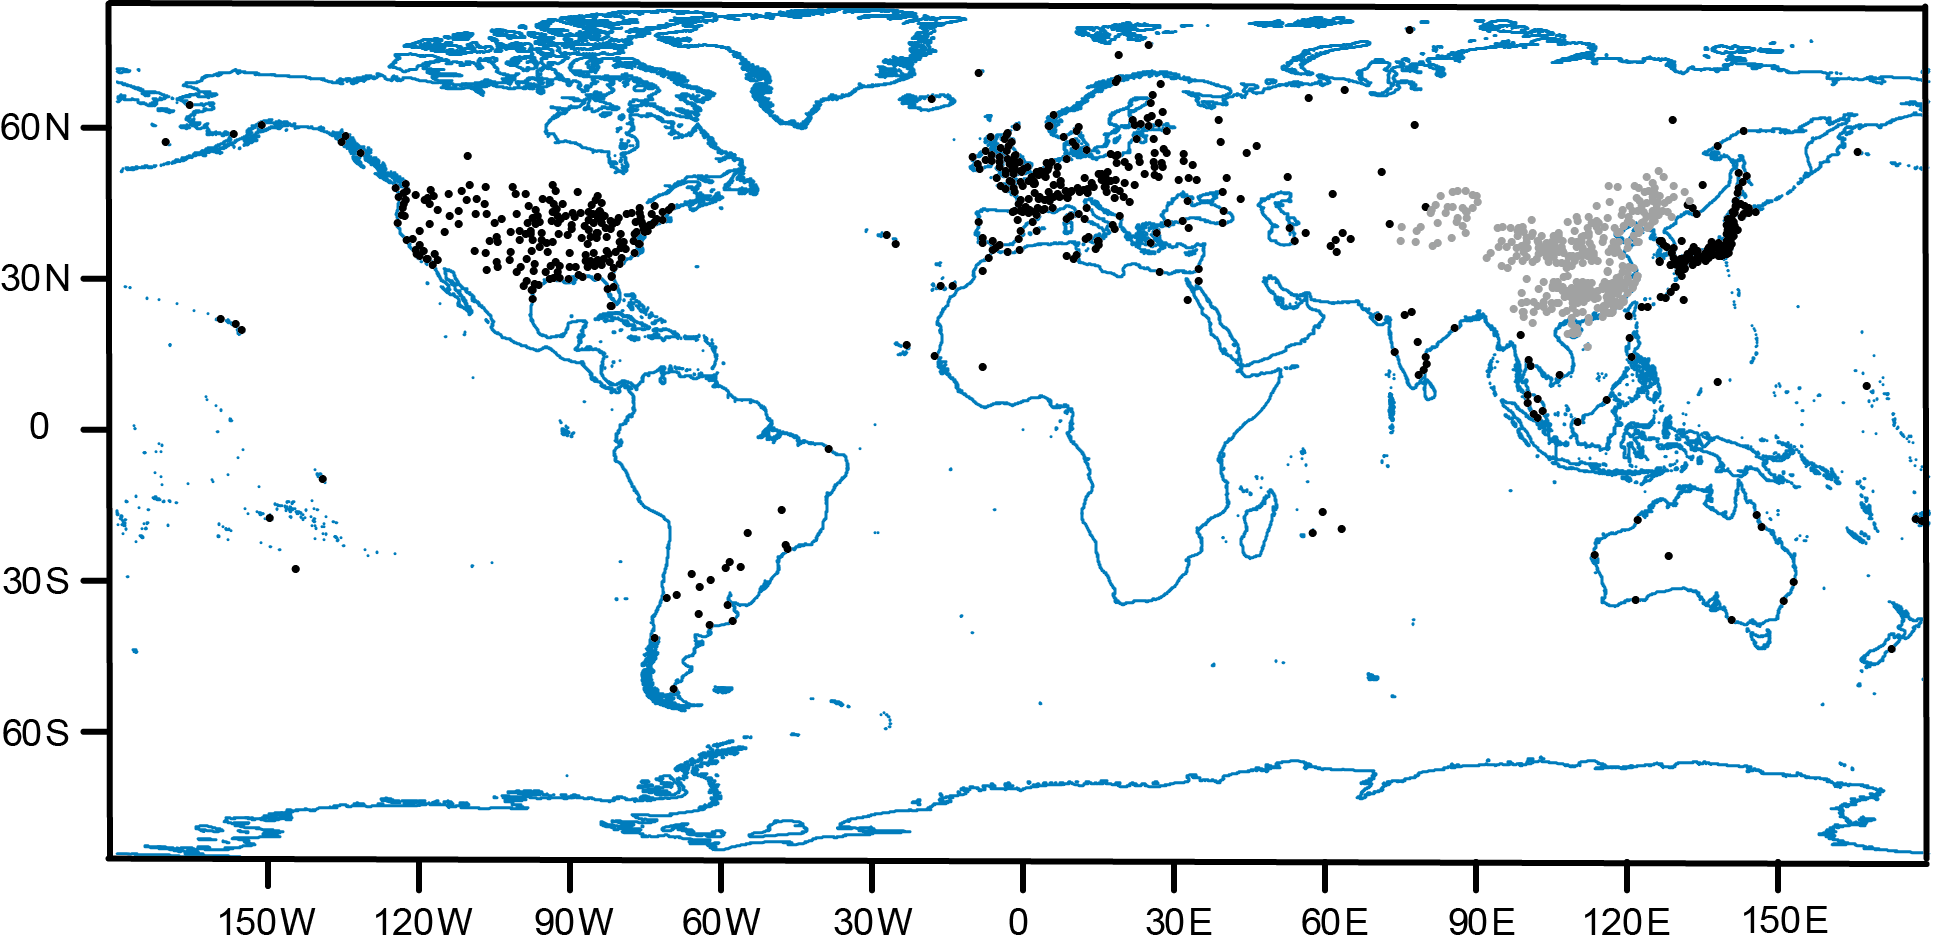
\includegraphics[width=0.7\textwidth]{NCEI_CMDC站点位置}
    \bicaption{NCEI-CMDC站点分布,黑色为NCEI站点,灰色为CMDC站点。}{Locations of NCEI-CMDC stations, black denotes NCEI stations, grey denotes CMDC stations. }
    \label{fig:NCEI_CMDCstations}
\end{figure}

本章中使用了以下5套再分析数据集与观测数据进行对比:

\begin{enumerate}
\item NCEP/NCAR再分析资料\citep{kalnay1996the}的水平分辨率为$2.5 \times 2.5$度,有28个垂直层次。其地表粗糙度的数据不随时间变化,且陆地地表风速未被同化,10 $m$风速是由模式最底层的风速根据Monin-Obukhov相似理论外插得到。NCEP/NCAR使用的模式在近地面100 $hPa$内有5个垂直层次,最底层为$\sigma = 0.995$。本章研究使用了6小时分辨率10 $m$ U、V风场资料。
\item NCEP-DOE再分析资料\citep{kanamitsu2002ncep–doe}的水平分辨率为$1.9 \times 1.9$度,垂直层次与NCEP/NCAR相同,为28个。其同化的数据也与NCEP/NCAR一致,只是算法上有所改进。与地表风速相关的改进包括地形平滑和边界层参数化方案以及土壤湿度的参数化。10 $m$风速的获得与NCEP/NCAR一致。本章研究使用了6小时分辨率10 $m$ U、V风场资料。
\item ERA-Interim再分析资料\citep{dee2011the}的水平分辨率为$ 0.75 \times 0.75$ 度,60个垂直层次。其同化了海表风速,但没有同化陆地地表风速。10 m风速同样是由模式最底层的风速根据Monin-Obukhov相似理论外插得到。本章使用了6小时分辨率10 $m$ U、V风场资料。
\item MERRA-2再分析资料\citep{molod2014development}的水平分辨率为0.5纬度$\times$ 0.625经度,72个垂直层次 。其同化了海表风速,但没有同化陆地地表风速。10 $m$风速的计算方式与前面提到的几套再分析资料类似。本章使用了1小时分辨率10 $m$ U、V风场资料。
\item JRA-55再分析资料\citep{kobayashi2015the}的水平分辨率为$ 1.25 \times 1.25$度,60个垂直层次。JRA-55同化了陆地地表风速资料,但仅用于近地面层(screen level)的分析,不会用于大气模式。10 $m$风速的由模式最底层风速根据单变量二维最优插值得到。本章使用了6小时分辨率10 $m$ U、V风场资料。
\end{enumerate}

本章中线性趋势的计算使用基于最小二乘方法的线性回归,计算方法如下:

建立线性回归模型:
\begin{equation} \label{eq:linearregression}
y = \beta_{0} + \beta_{1}x + \varepsilon
\end{equation} 
其中$\beta_{0}$和$\beta_{1}$为回归系数($\beta_{1}$即为“趋势”),$x$为回归量,$y$为回归子, $\varepsilon$为残差,为使得残差平方和最小,
\begin{equation} 
 \pmb{\beta} = \left( X^{T}X \right)^{-1} X^{T} Y 
\end{equation} 
$X$为回归量矩阵,$ \pmb{\beta} $为回归系数向量,$Y$为回归子向量。

统计显著性检验使用双侧t检验。突变点检测使用滑动t检验,人为设置某一时刻为基准点,t统计量计算方法为:

\begin{equation} \label{eq:mvttest}
t = \frac{\bar{x_{1}} - \bar{x_{2}}}{ s \sqrt{\frac{1}{n_{1}} + \frac{1}{n_{2}}}}
\end{equation} 
其中,
\begin{equation} 
s = \sqrt{\frac{n_{1}\sigma_{1}^{2} + n_{2}\sigma_{2}^{2}}{n_{1} - n_{2} - 2}}
\end{equation} ~\\
$\bar{x_{1}}$、$\bar{x_{2}}$分别为基准点前后子序列均值,$\sigma_{1}$ 、$\sigma_{2}$  为子序列标准差,$n_{1}$ 、$n_{2}$为子序列样本数量,对比$t$统计量与$t$分布临界值大小确定突变点的显著性水平。

\section{北半球陆地地表风速长期线性趋势}\label{sec:NHwindchange}

\subsection{陆地地表风速长期线性趋势的空间特征}

\begin{figure}[!t]
    \centering
    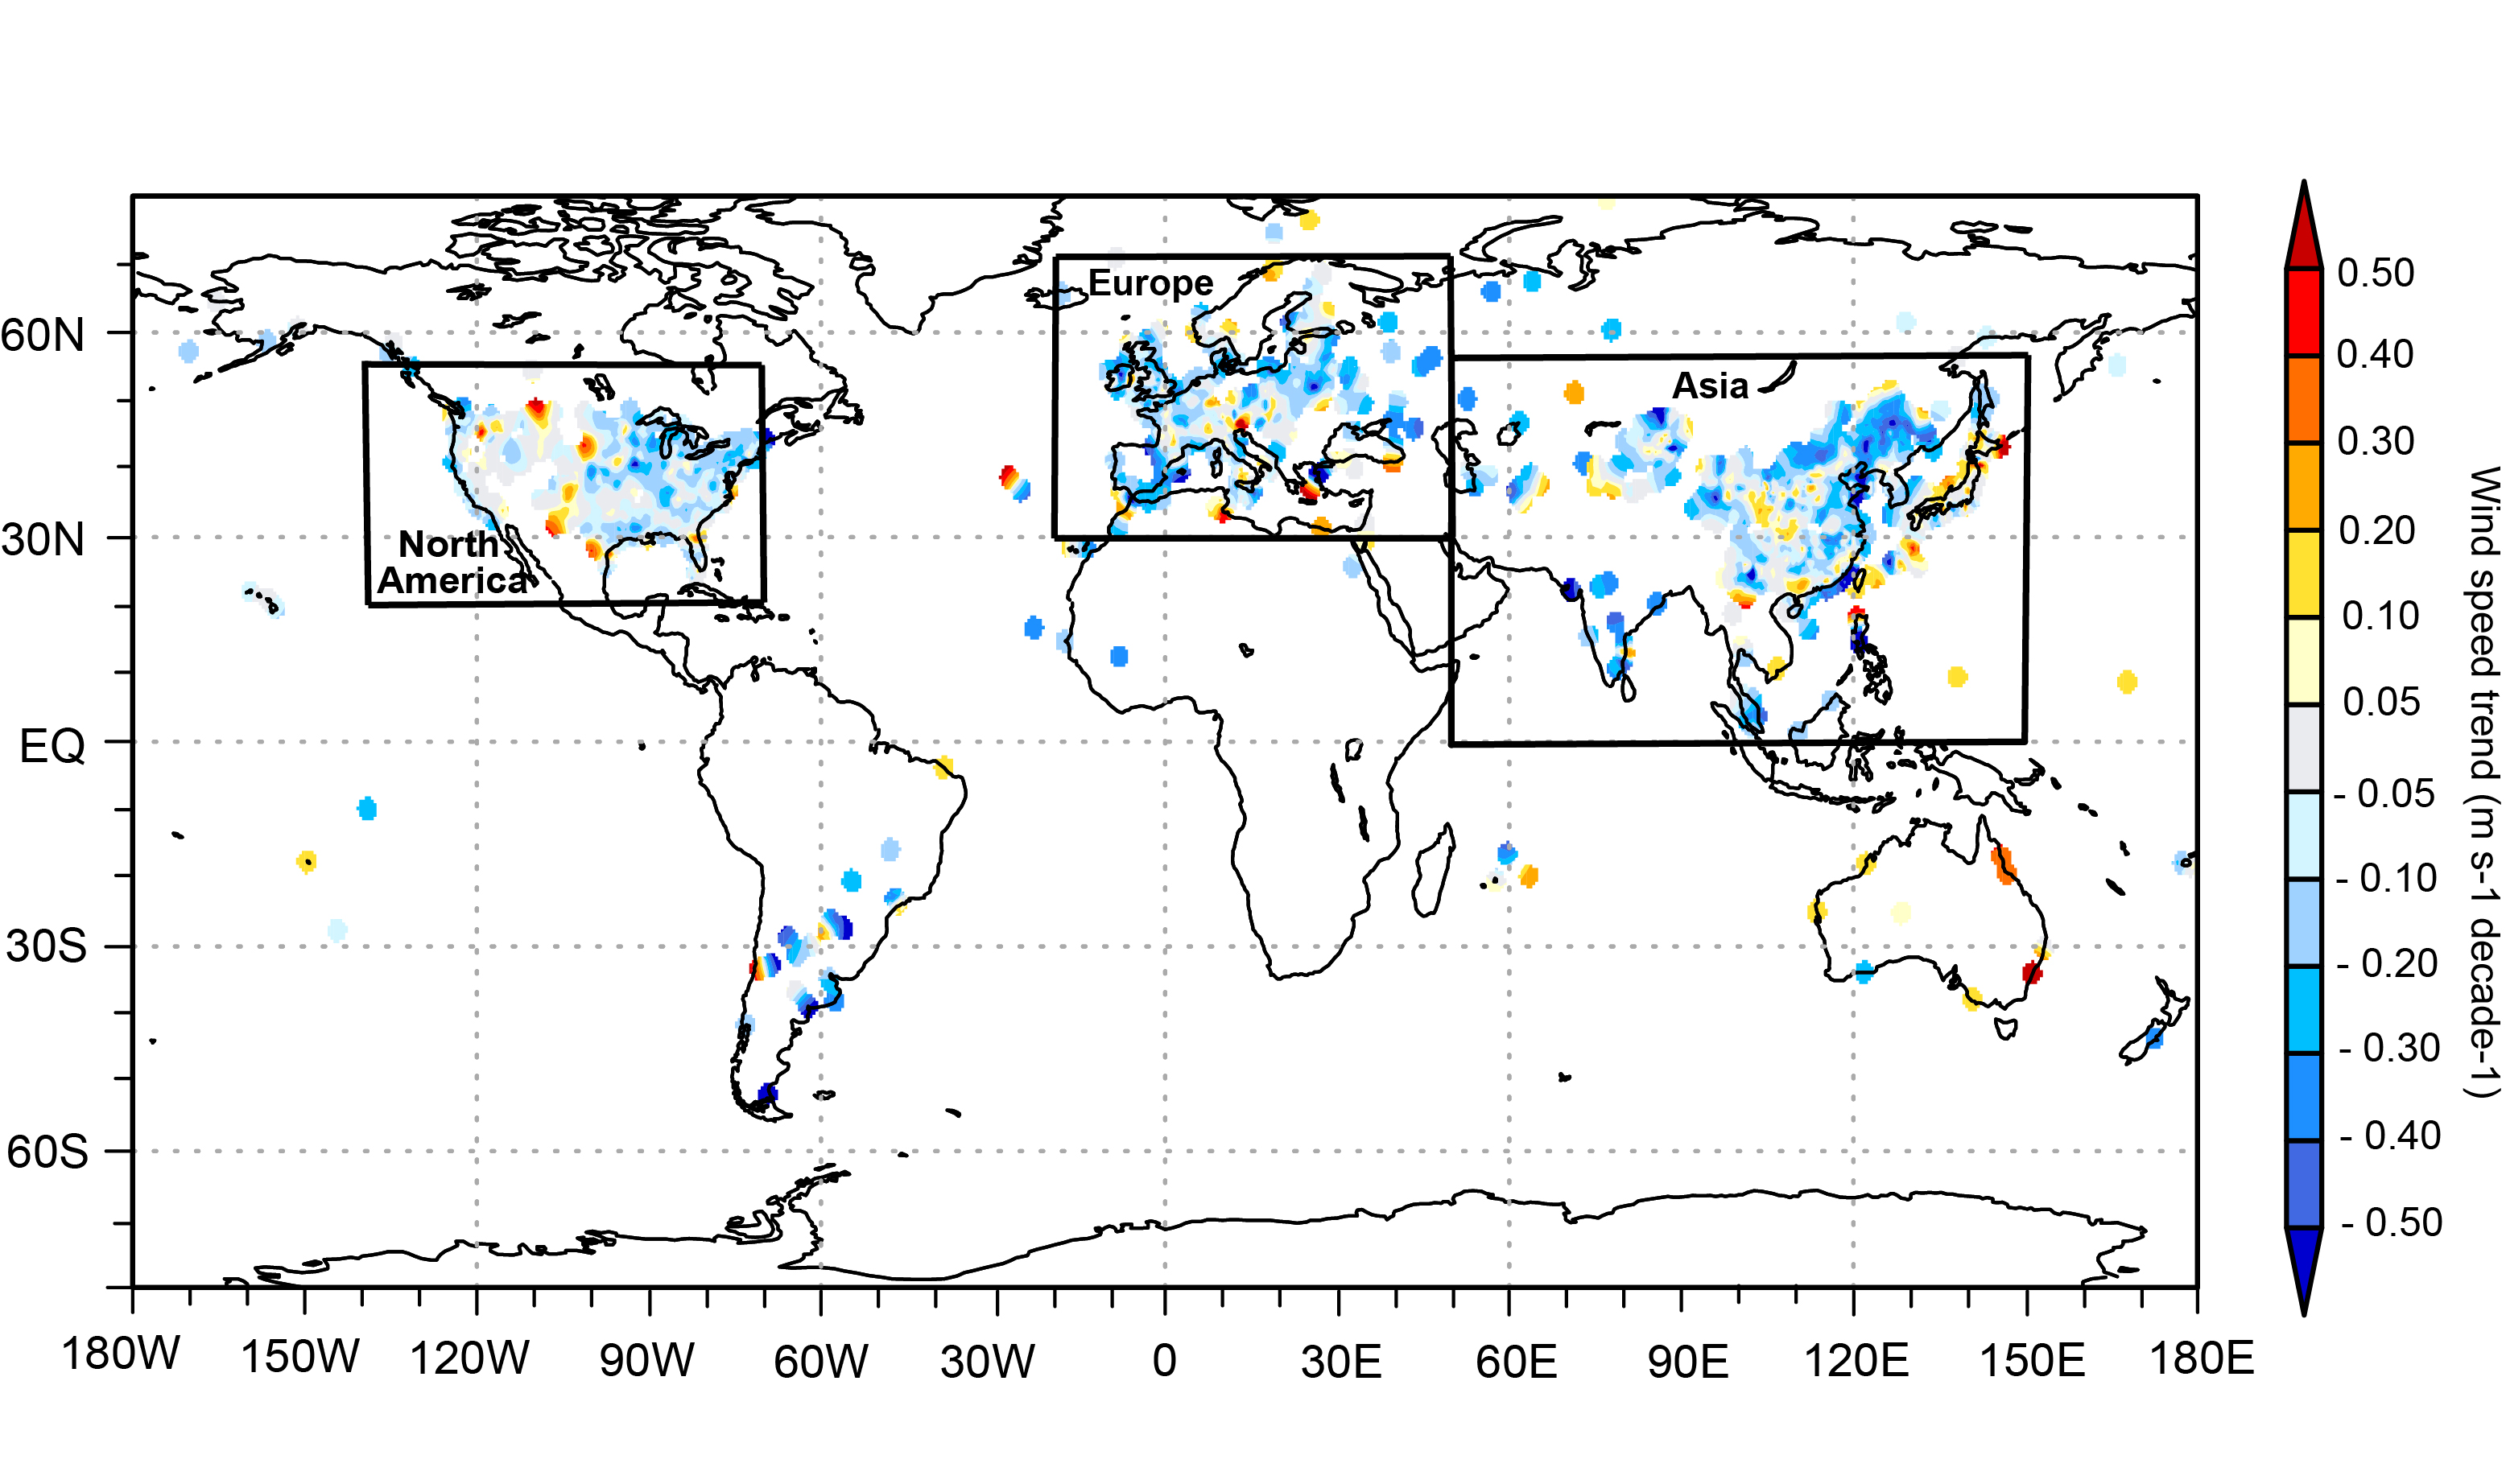
\includegraphics[width=1\textwidth]{全球年平均风速长期趋势}
    \bicaption{全球年平均风速长期趋势($m ~ s^{-1}$每十年)。图中三个框出的区域的范围分别为:北美洲 20-55 N,50-140 W;欧洲 30-70 N,20W-50 E;亚洲0-55 N,50-150 E。}{Long-term linear trends of annual mean wind speed across the globe (in $m ~ s^{-1} ~ decade^{-1}$). The spatial ranges of the framed areas are North America 20-55 N, 50-140 W, Europe 30-70 N, 20W-50 E, Asia 0-55 N, 50-150 E. }
    \label{fig:NHwindtrend}
\end{figure}

对NCEI-CMDC地表风速的年平均值进行线性回归,得到全球(主要是北半球)1979-2016年陆地地表风速的长期趋势。结果发现,全球有73\%的站点风速出现了下降趋势,其中有67\%显著下降(p < 0.01),中位数风速趋势为$ -0.081 ~ m ~ s^{-1}$每十年。将大部分观测站点分布的北半球分为三个区域:北美洲(20-55 N,50-140 W),欧洲(30-70 N,20 W-50 E)和亚洲(0-55 N,50-150 E)分别进行分析,得到这三个地区中位数风速趋势分别为-0.075,-0.105和-0.075 $m ~ s^{-1}$每十年,即在38年中分别累计变化了-6.5\%,-9.6\%和-11.2\%。值得一提的是,中国的中位数风速趋势为-0.110 $m ~ s^{-1}$每十年,累计变化-17.5\%(图 \ref{fig:NHwindtrend})。这些结果与前人的研究具有较高的一致性(第\ref{chap:intro}章\;表 \ref{tab:globalwindtrend})。这里使用中位数而不是平均数,因为中位数相比平均数具有更好的鲁棒性,即更不容易受到极端值的影响,因而更适合于反映一个区域整体的状况,以下的许多分析也是基于中位数来进行。

\begin{figure}[!b]
    \centering
    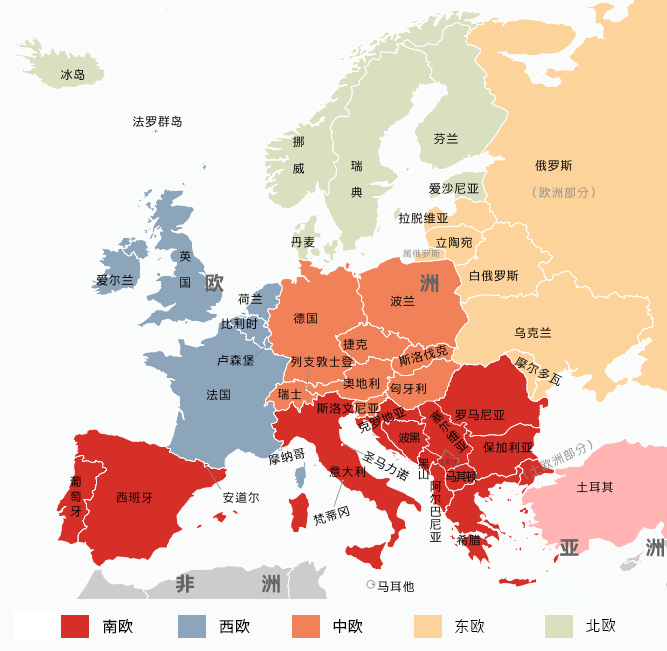
\includegraphics[width=0.45\textwidth]{欧洲分区}
    \bicaption{欧洲分区图}{European Zoning Map}
    \label{fig:EU}
\end{figure}

不同地区的地表风速长期趋势表现出了较大的差别。在北美洲,美国中北和东北地区风速下降最为明显,大部分站点趋势值小于-0.1 $m ~ s^{-1}$每十年;与之相对的,美国落基山脉地区多数站点风速趋势接近为0,个别站点出现了风速增强的情况;美国西海岸一线表现出了一定程度的风速下降,多数站点在-0.2 \textasciitilde -0.05 $m ~ s^{-1}$每十年。在欧洲,西欧地区(欧洲分区见图 \ref{fig:EU})有较为明显的风速下降;中欧地区,奥地利和斯洛文尼亚有较为明显风速上升,波兰中部风速有较为明显的下降,其他大部分地区没有明显的风速趋势;南欧地区,西班牙和葡萄牙风速有明显的上升;东欧地区大部分站点都表现了较为明显的风速下降。亚洲地区,印度风速下降明显,大部分站点趋势值小于-0.2 $m ~ s^{-1}$每十年;中国风速下降明显的地区是中国东北、华北和西北地区,中部地区部分站点风速有一定程度上升;日本风速部分站点风速明显下降,部分站点风速明显上升,二者数量大致相同(图 \ref{fig:NHwindtrend})。

\subsection{百分位风速长期线性趋势}

\begin{figure}[!hb]
    \centering
    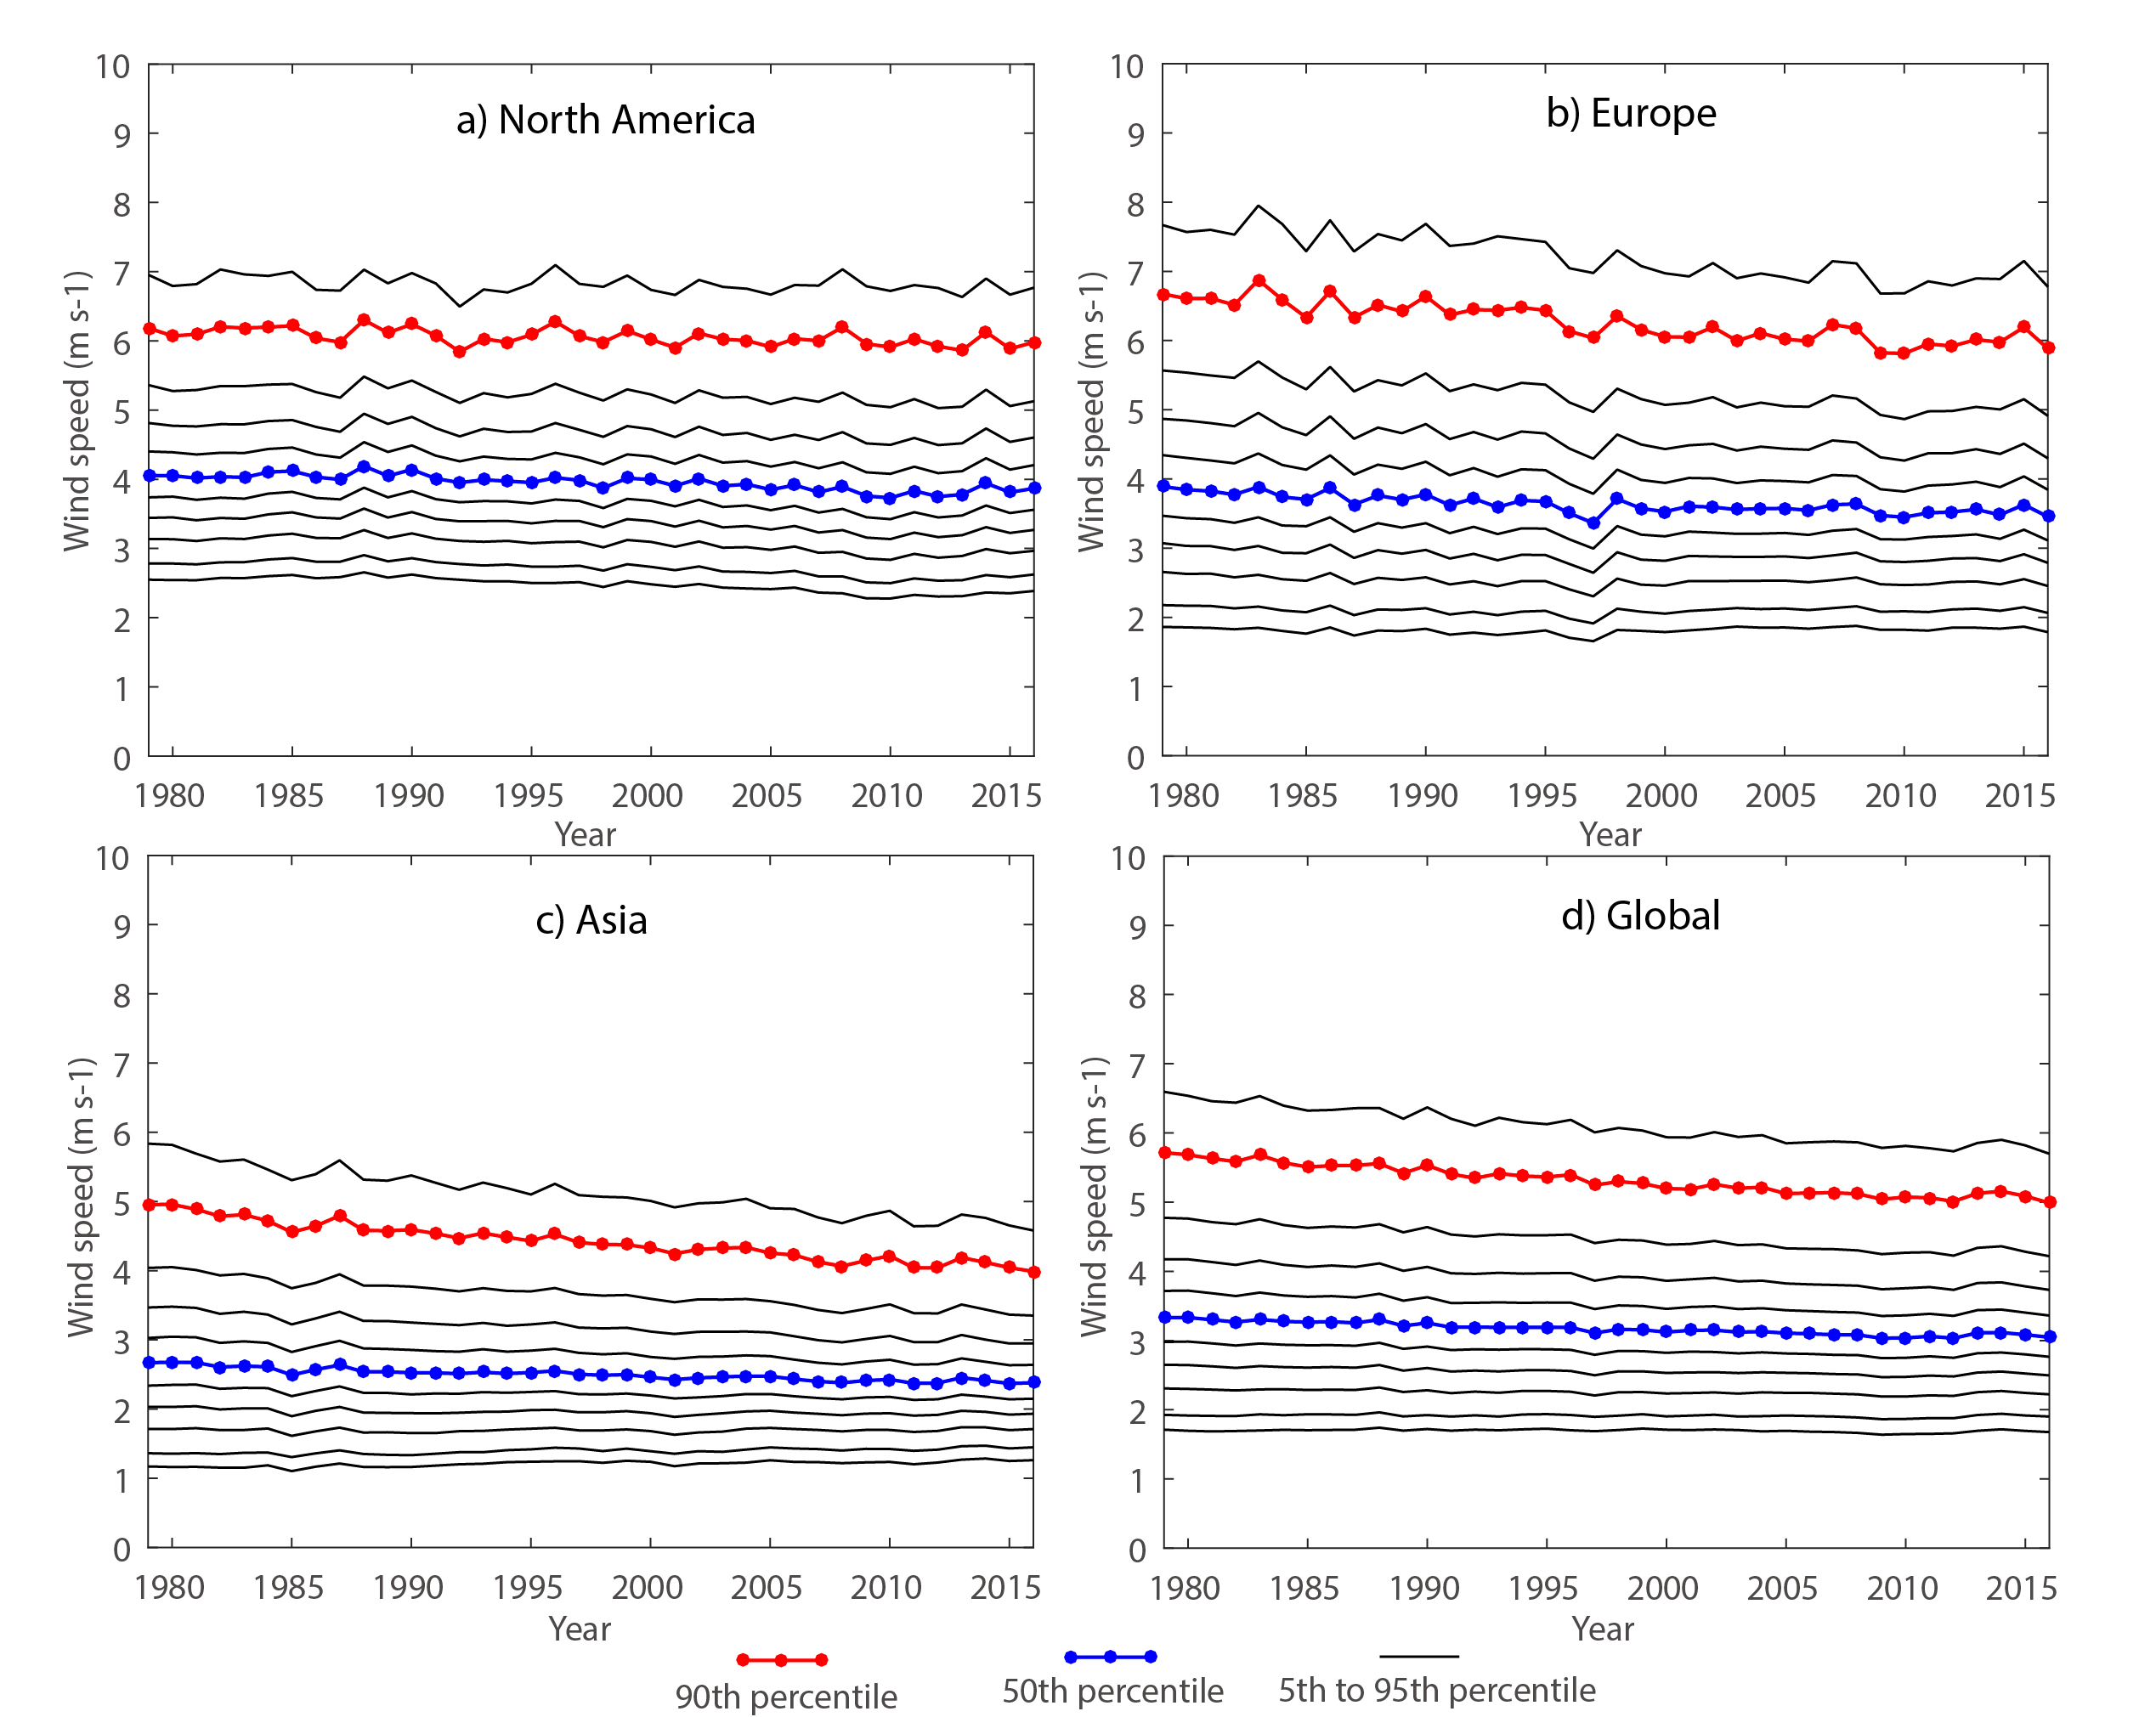
\includegraphics[width=1\textwidth]{百分位风速的演变}
    \bicaption{百分位风速的演变($m ~ s^{-1}$)。a)北美洲,b)欧洲,c)亚洲,d)全球。红色为90百分位,蓝色为50百分位,黑色为5、10、20、...、80、90、95百分位。}{Evolution of wind speeds at different percentiles (in $m ~ s^{-1}$). a) North America, b)Europe, c)Asia, d)Global. Red line denotes winds at 90 percentile, blue denotes 50 percentile, black denotes 5, 10, 20, ..., 80, 90, 95 percentile.}
    \label{fig:windpercentile}
\end{figure}

不同百分位风速变化也有不同特点。全球平均来看,大风下降快于小风(图 \ref{fig:windpercentile} d),表 \ref{tab:windpercentile})。各大洲分别来看,在北美洲,低百分位风速(即小风)下降快于高百分位风速(即大风)。5 - 40百分位风速的趋势约为-0.083 $m ~ s^{-1}$每十年,而80百分位风速趋势为-0.072 $m ~ s^{-1}$每十年,95百分位仅为-0.04 $m ~ s^{-1}$每十年。其中有部分原因可能是美国1990年代安装的ASOS观测系统测量的大风比之前观测系统偏大,而小风偏小\citep{mckee2000climate}。然而,在北美百分位风速演变中并未看到1990年代各百分位有显著变化,说明观测仪器变化的影响不是非常明显(图 \ref{fig:windpercentile} a),表 \ref{tab:windpercentile})。在欧洲,风速越大越趋向于减弱。5百分位风速略有上升,为0.008 $m ~ s^{-1}$每十年,从10百分位开始风速出现下降,到50百分位趋势达到了-0.093 $m ~ s^{-1}$每十年,90百分位下降速度超过了50百分位的两倍,达到了-0.218 $m ~ s^{-1}$每十年(图 \ref{fig:windpercentile} b),表 \ref{tab:windpercentile})。亚洲的情况与北美洲类似,5–20 百分位风速略有上升趋势,而从30百分位开始风速开始下降,50百分位趋势达到-0.074 $m ~ s^{-1}$每十年,90百分位达到-0.237 $m ~s^{-1}$每十年(图 \ref{fig:windpercentile} c),表 \ref{tab:windpercentile})。因为风力发电机只可以利用较大的风速进行,通常需超过3 $m ~s^{-1}$,因而在欧洲和亚洲出现的大风减弱更快的状况对风力发电十分不利。

\begin{table}[!htbp]
    \bicaption{全球及各大洲百分位风速趋势($m ~ s^{-1}$每十年)}{Global and regional wind speed trends at different percentiles (in $m ~ s^{-1} ~ decade^{-1}$) }
    \label{tab:windpercentile}
    \centering
    \small% fontsize
    \setlength{\tabcolsep}{15 pt}% column separation
    \renewcommand{\arraystretch}{1.0}%row space 
    \begin{tabular}{lcccc}
        \hline
        地区 & 北美洲 & 欧洲 & 亚洲 & 全球 \\
        %\cline{2-9}% partial hline from column i to column j
        \hline
        5th & -0.084 & 0.080 & 0.028 & -0.010 \\
        10th & -0.084 & -0.006 & 0.027 & -0.008 \\
        20th & -0.083 & -0.028 & 0.003 & -0.023 \\
        30th & -0.082 & -0.049 & -0.021 & -0.040 \\
        40th & -0.082 & -0.071 & -0.047 & -0.057 \\
        50th & -0.082 & -0.093 & -0.074 & -0.076 \\
        60th & -0.081 & -0.114 & -0.101 & -0.095 \\
        70th & -0.078 &  -0.141 & -0.134 & -0.118 \\
        80th & -0.072 & -0.171 & -0.174 & -0.177 \\
        90th & -0.057 & -0.218 & -0.237 & -0.184 \\
        95th & -0.040 & -0.261 & -0.296 & -0.222 \\           
        \hline
    \end{tabular}
\end{table}

\subsection{四季风速长期线性趋势}

\begin{figure}[!b]
    \centering
    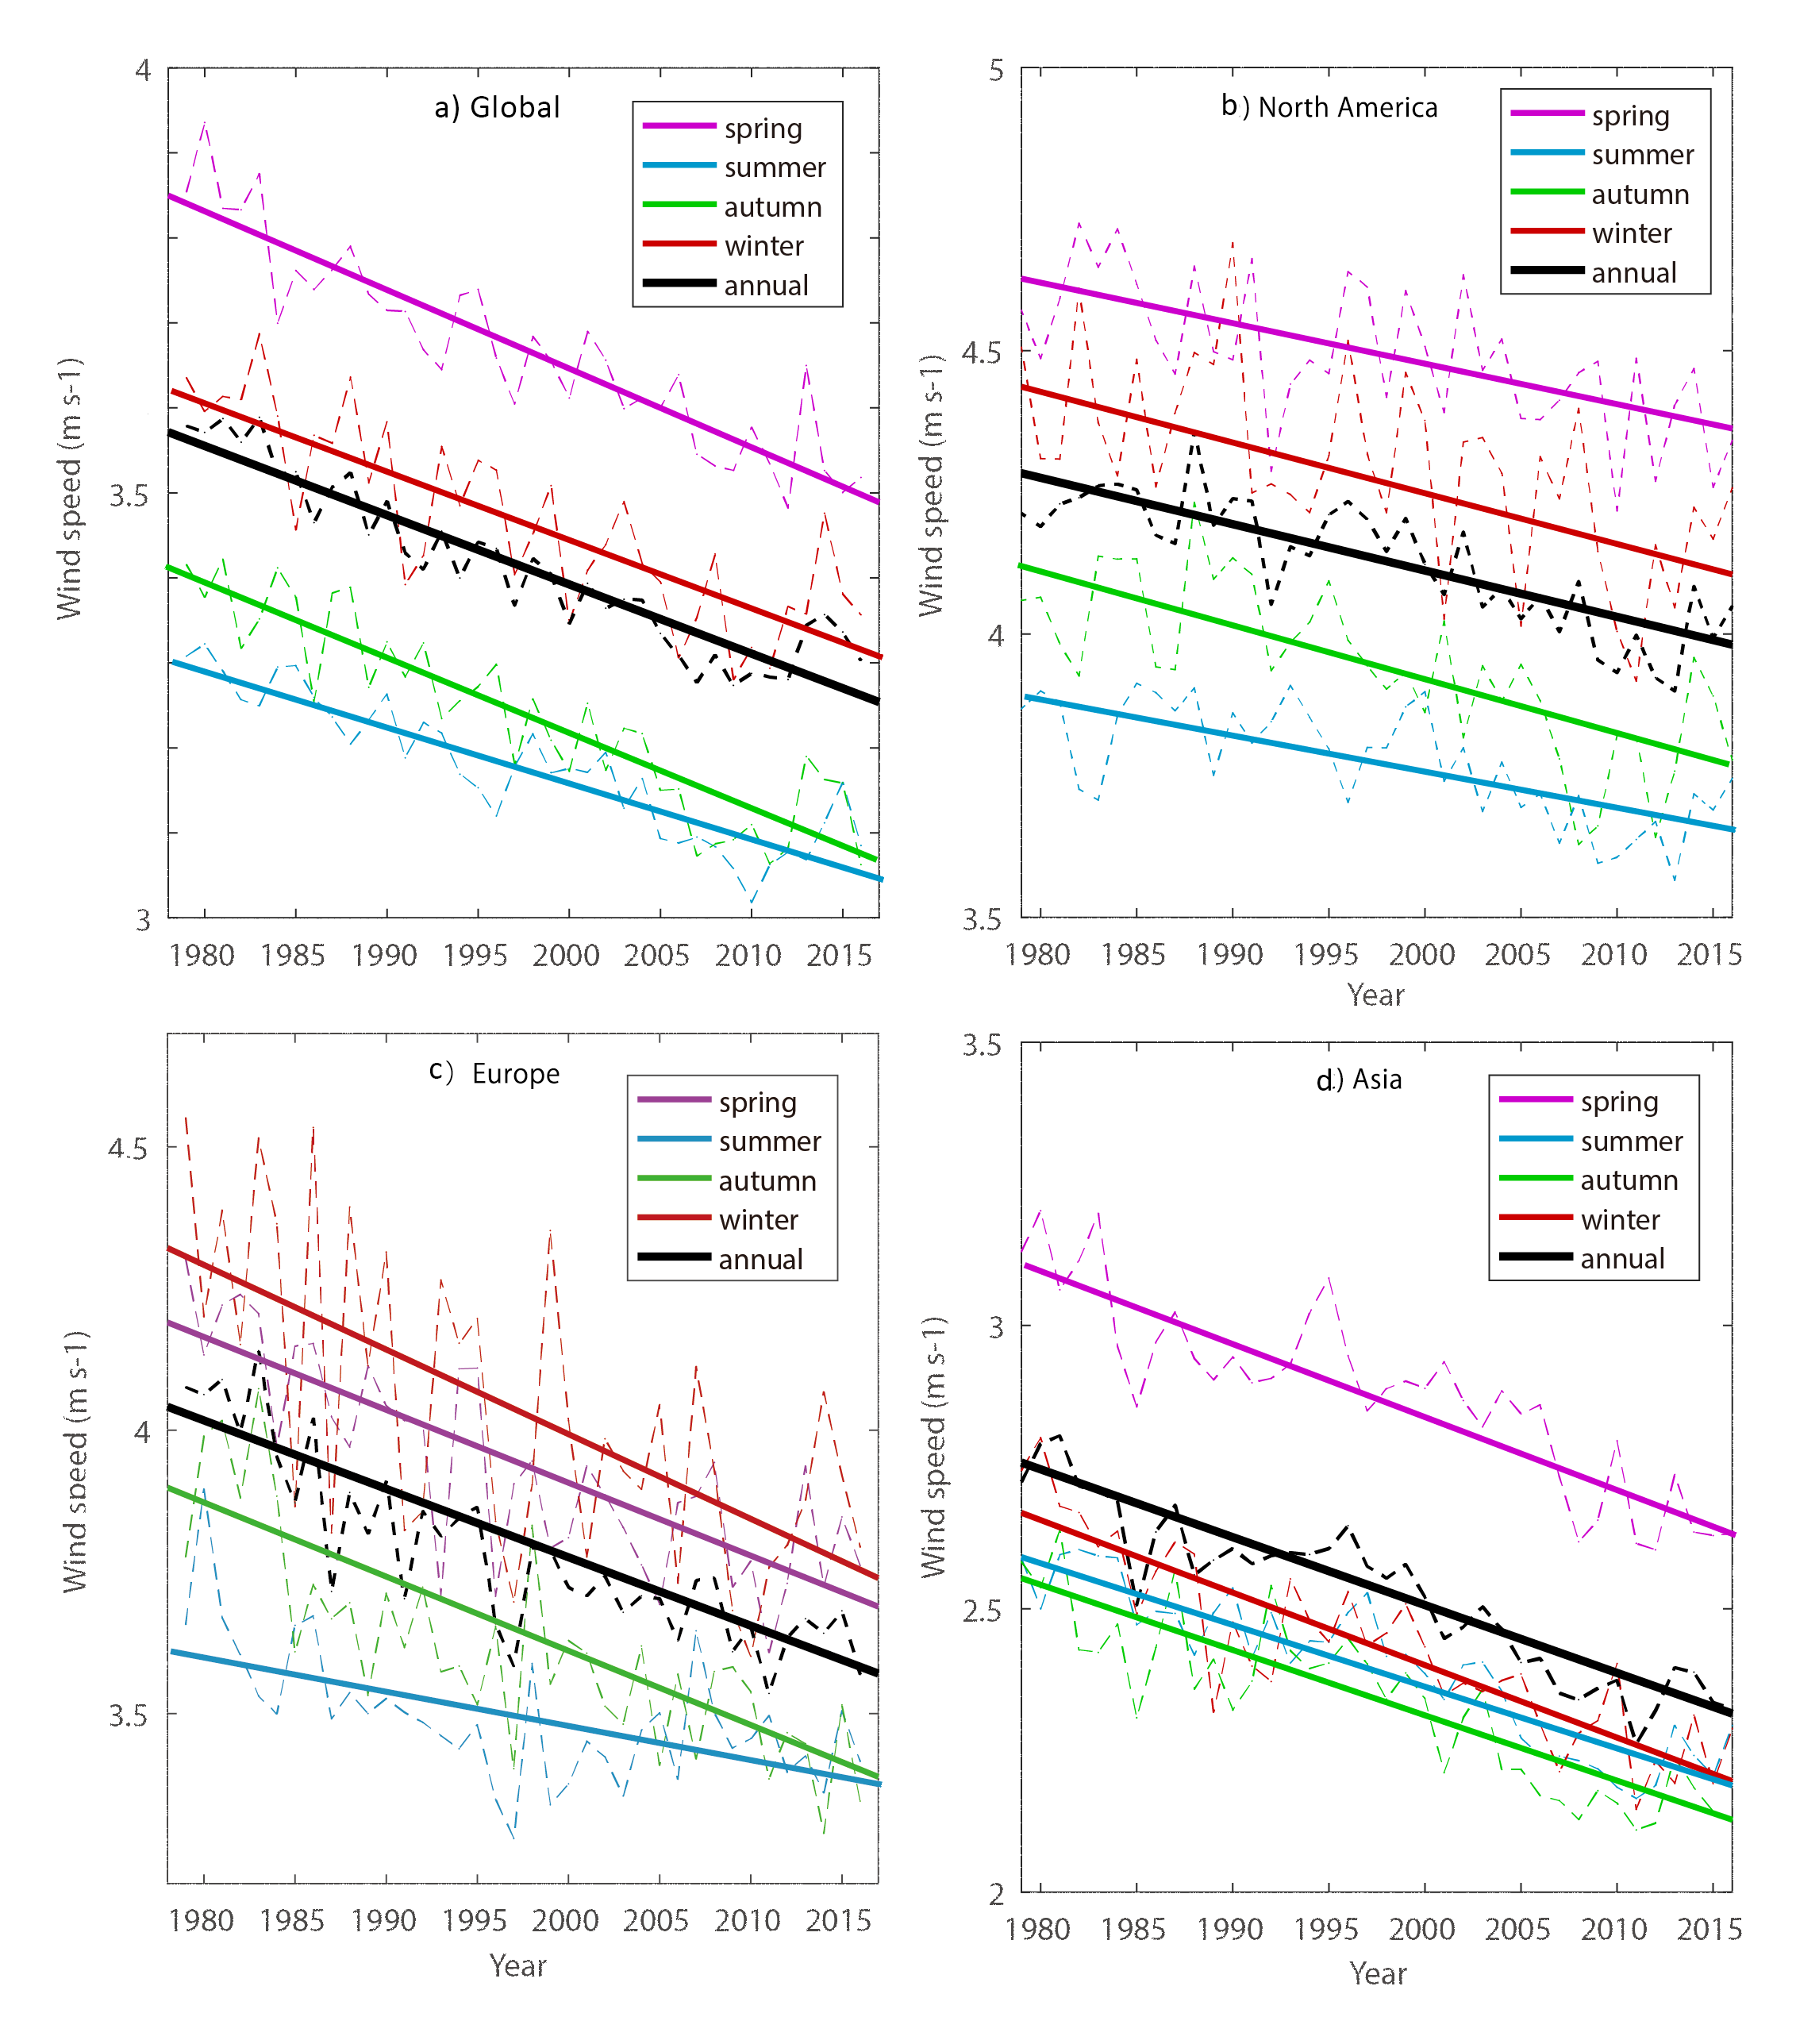
\includegraphics[width=0.9\textwidth]{各大洲中位数风速趋势}
    \bicaption{各大洲中位数风速趋势。a)全球,b)北美,c)欧洲,d)亚洲。紫色为春季,蓝色为夏季,绿色为秋季,红色为冬季,黑色为年平均。虚线为各年对应值,实线为虚线的线性趋势。}{Global and regional median wind speed trends. a)Global, b)North America, c)Europe, d)Asia. Purple color denotes spring, blue denotes summer, green denotes fall, red denotes winter, black denotes annual mean. Dash line denotes value for every year, soild line is linear trend line of dash line.}
    \label{fig:regionalmedianwindtrend}
\end{figure}

\begin{figure}[!b]
    \centering
    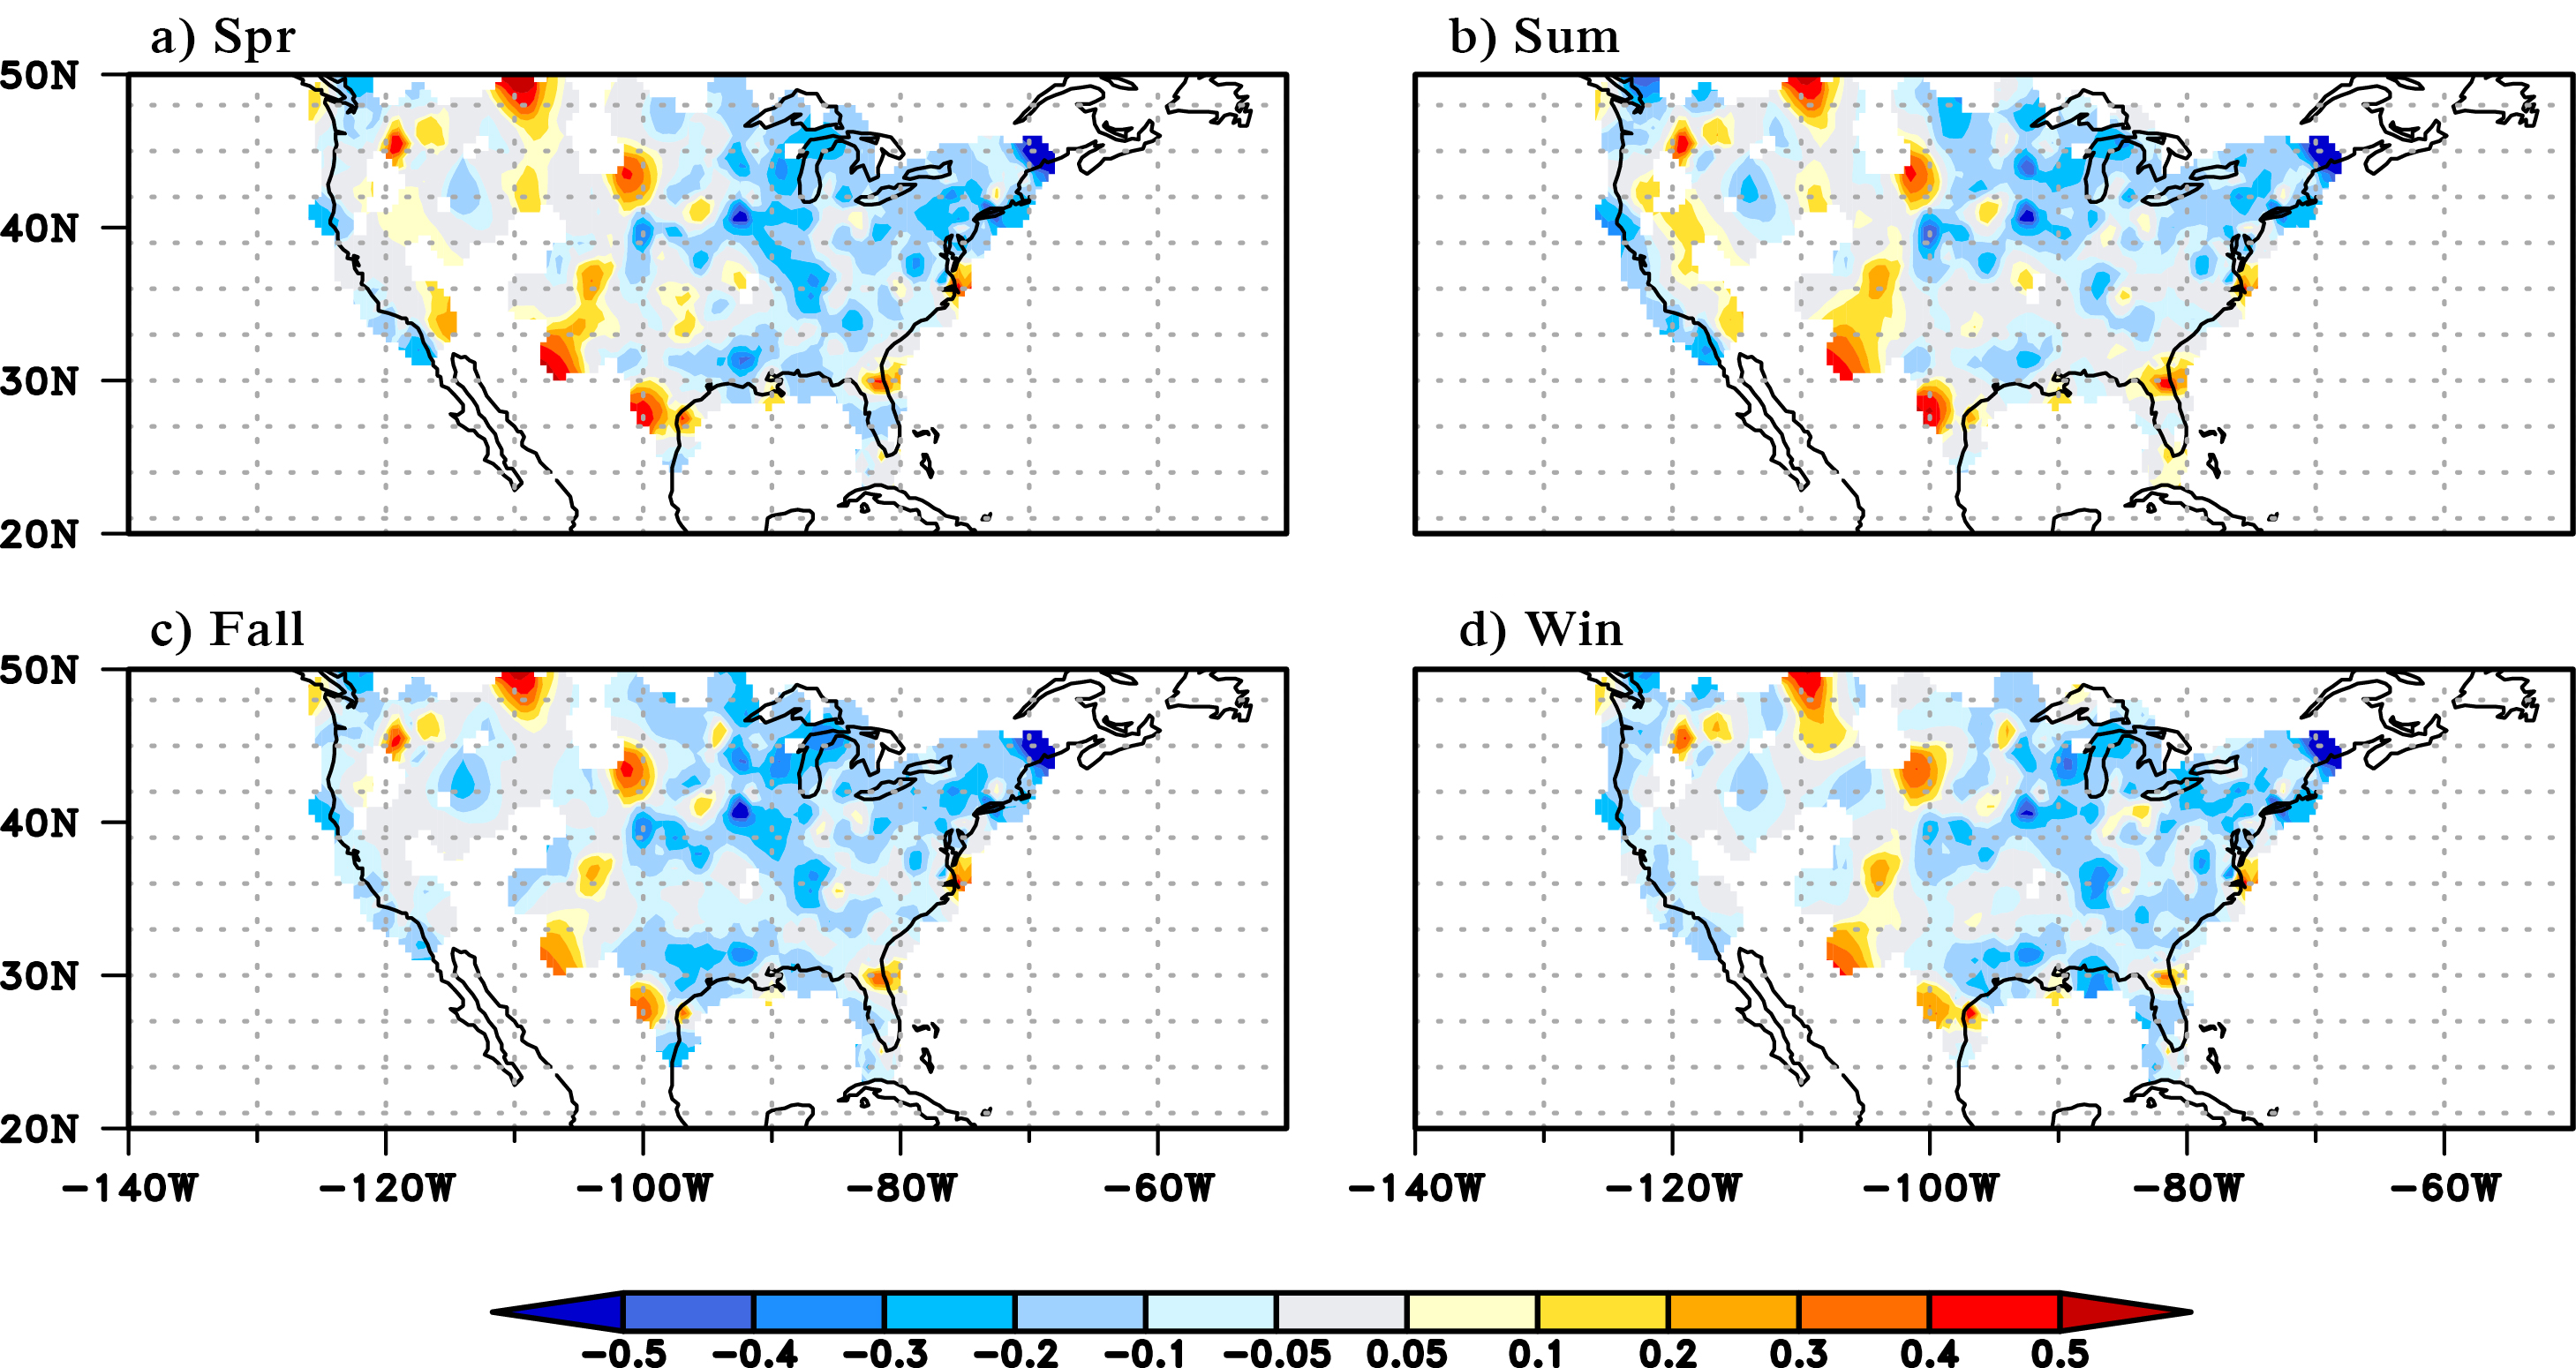
\includegraphics[width=0.8\textwidth]{北美洲四季风速长期趋势}
    \bicaption{北美四季风速长期趋势 ($m ~ s^{-1}$每十年)。a)春季(3-5月),b)夏季(6-8),c)秋季(9-11月),d)冬季(12月-次年2月)}{Long-term seasonal wind speed trends over North America (in $m ~ s^{-1} ~ decade^{-1}$). a) Spring (March to May), b) Summer (June to August), c) Fall (September to November), d) Winter (December to next February).}
    \label{fig:NAwindtrend}
\end{figure}

\begin{figure}[!htbp]
    \centering
    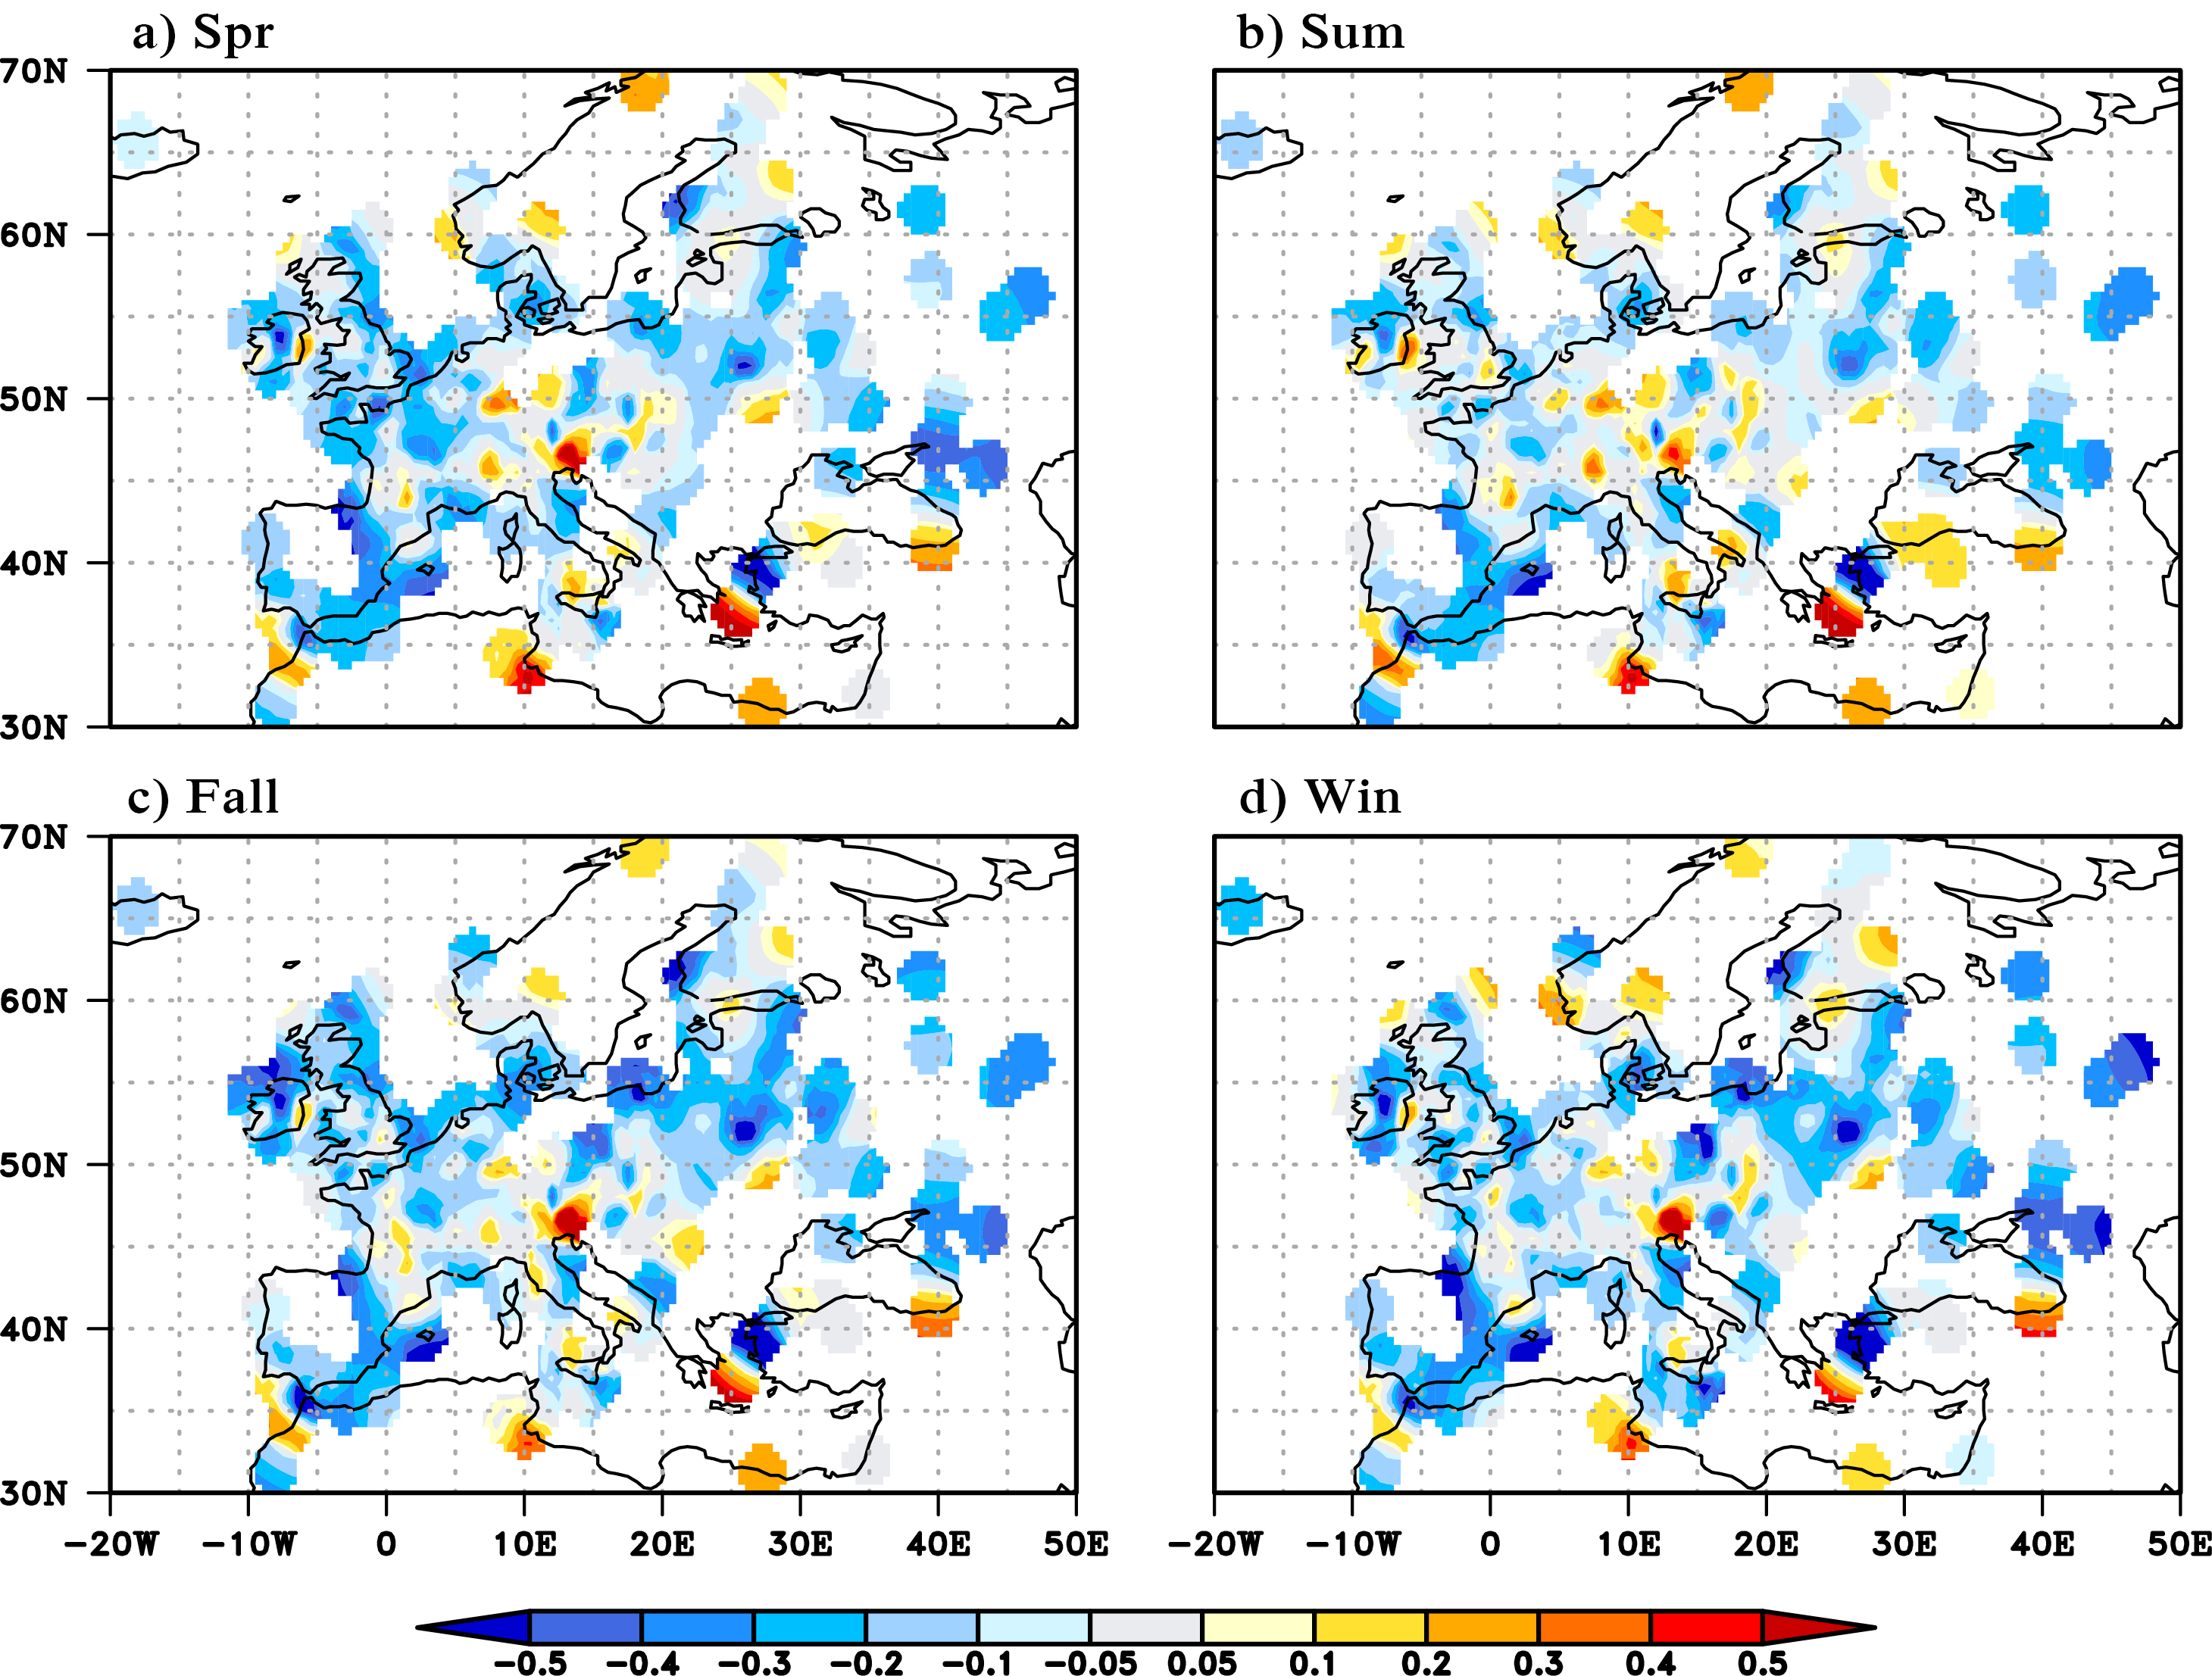
\includegraphics[width=0.75\textwidth]{欧洲四季风速长期趋势}
    \bicaption{欧洲四季风速长期趋势。与图 \ref{fig:NAwindtrend} 类似。}{Same as Figure \ref{fig:NAwindtrend}, but for Europe.}
    \label{fig:EUwindtrend}
\end{figure}

\begin{figure}[!htbp]
    \centering
    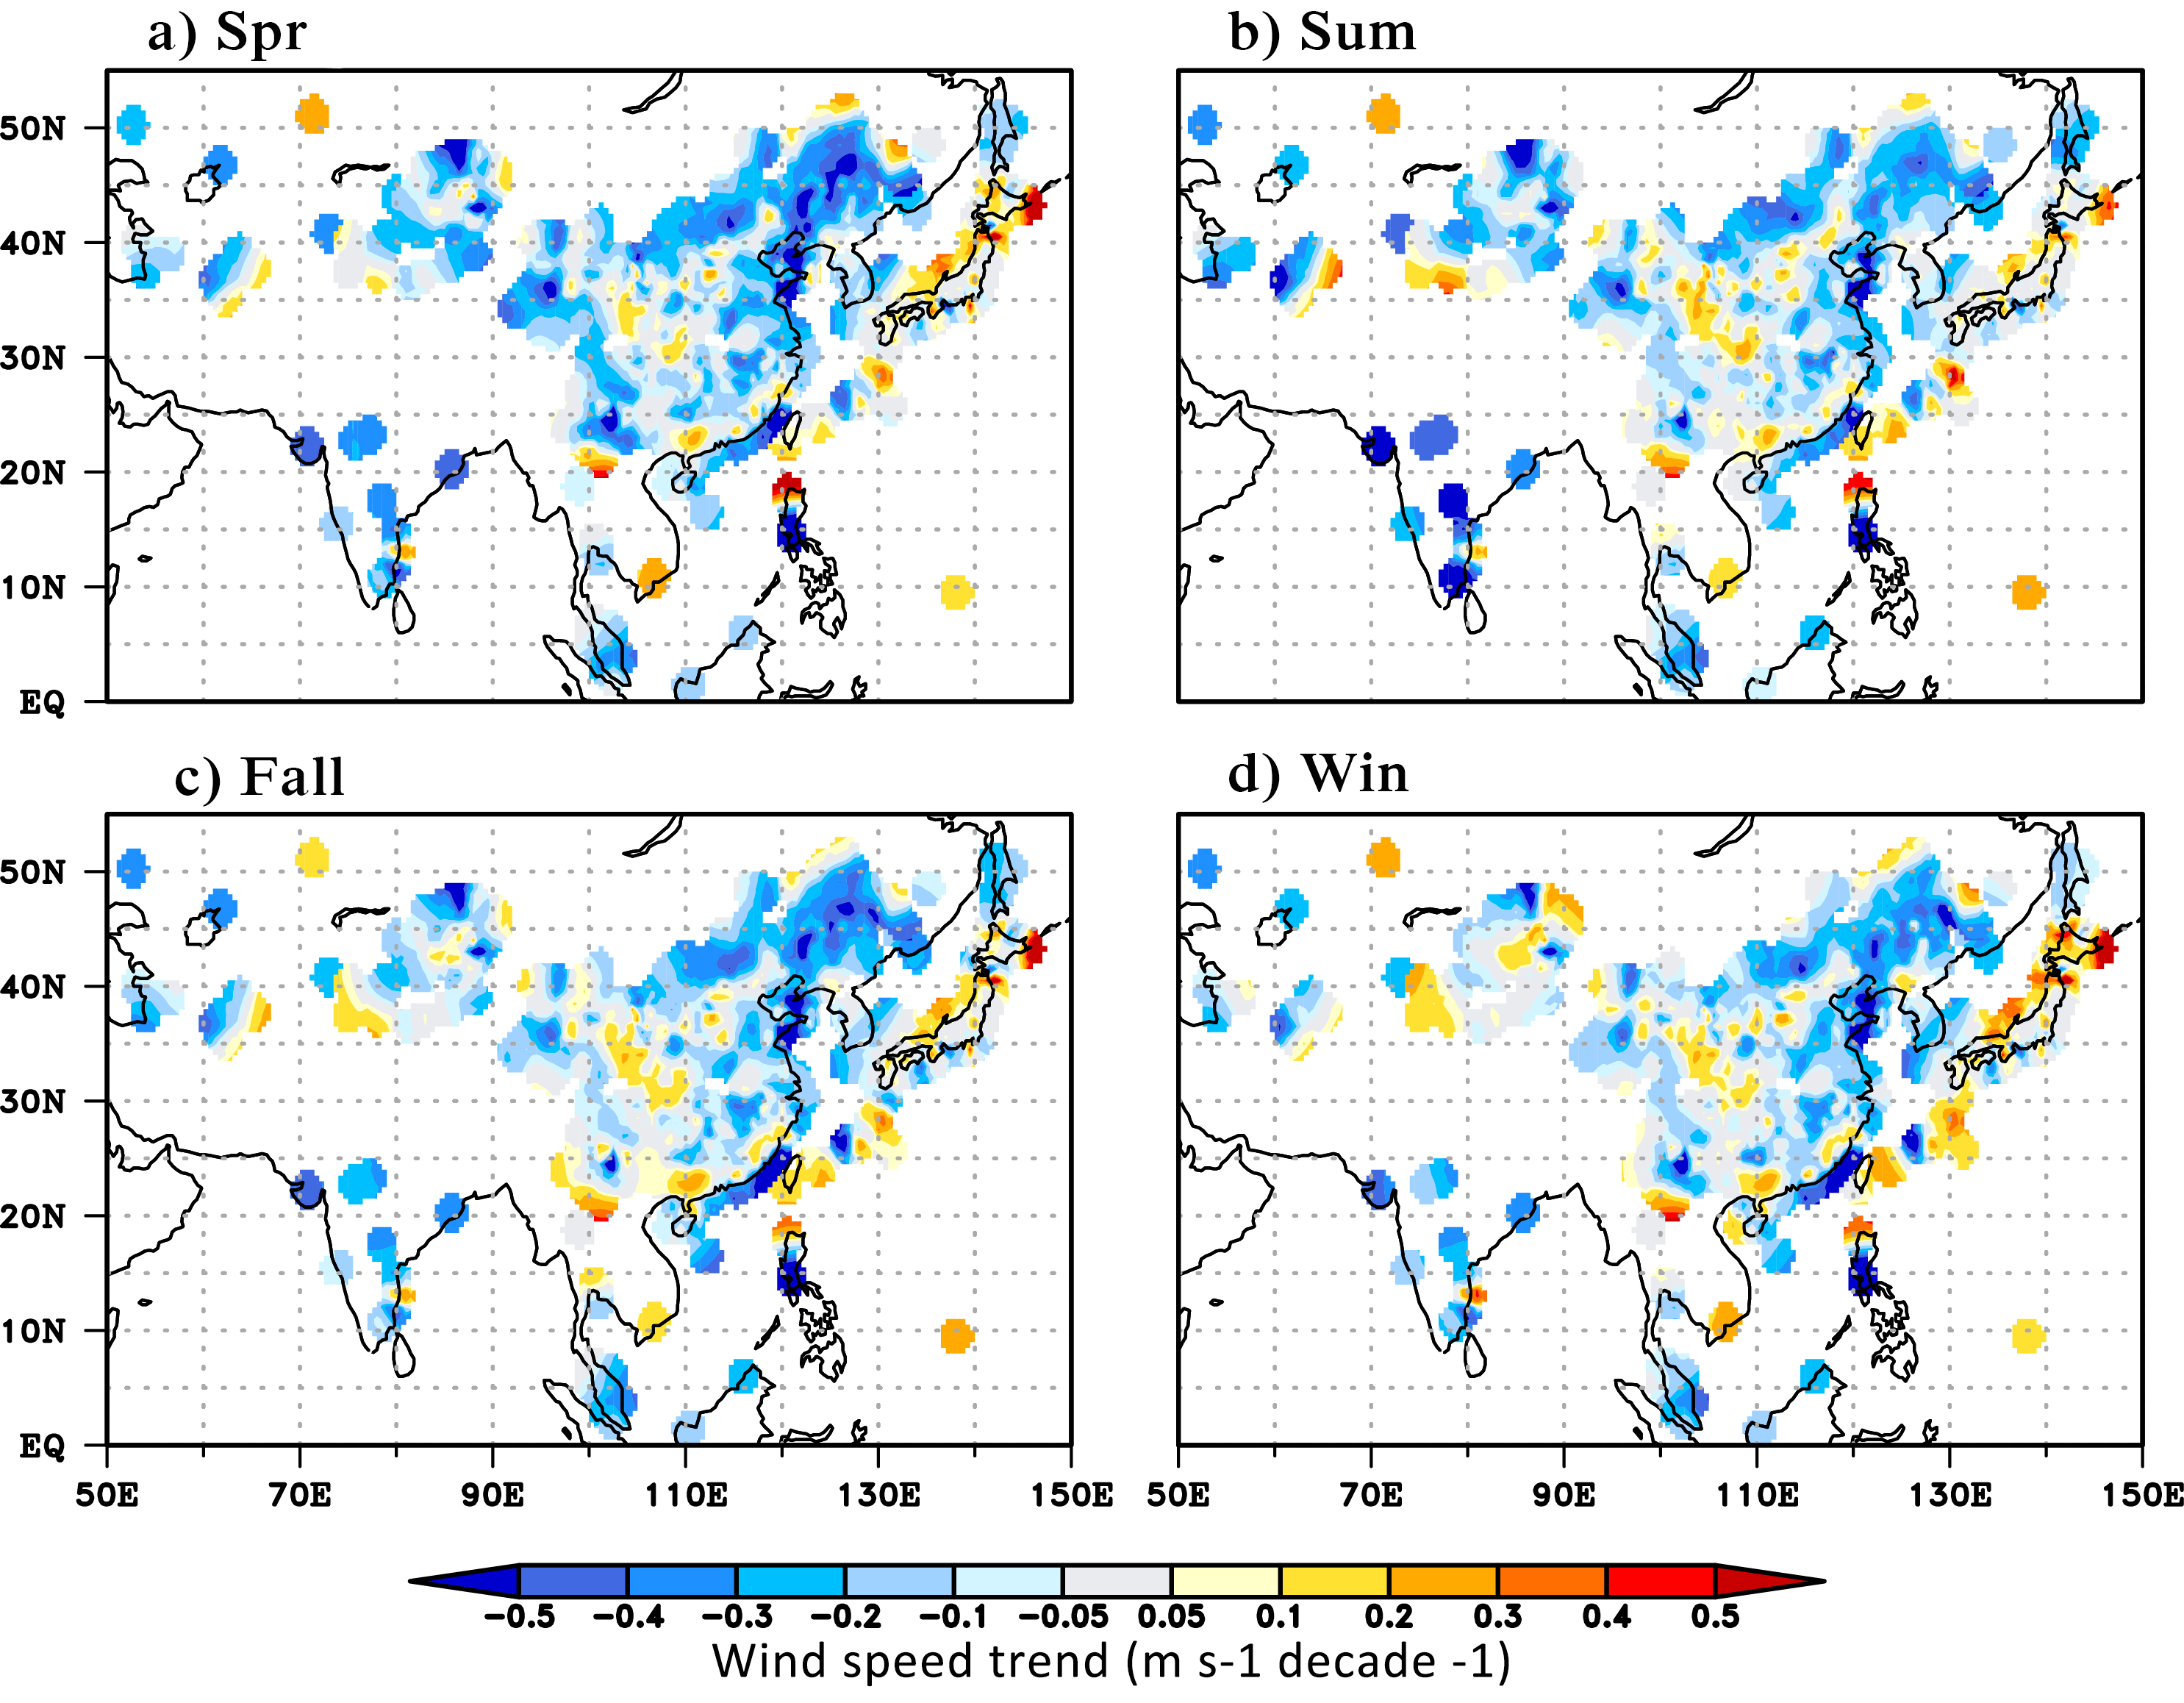
\includegraphics[width=0.75\textwidth]{亚洲四季风速长期趋势}
    \bicaption{亚洲四季风速长期趋势。与图 \ref{fig:NAwindtrend} 类似。}{Same as Figure \ref{fig:NAwindtrend}, but for Asia.}
    \label{fig:ASwindtrend}
\end{figure}

将一年划分为四个季节,分别是春季(3-5月)、夏季(6-8月)、秋季(9-11月)和冬季(12月至次年2月),风速在不同季节的长期线性趋势有一定差异。全球平均来看,平均风速和趋势的季节间差异明显,春季平均风速最大同时下降最快(-0.089 $m ~ s^{-1}$每十年),夏季平均风速最小同时下降最慢(-0.065 $m ~ s^{-1}$每十年)(图 \ref{fig:regionalmedianwindtrend} a))。在北美洲,平均风速春季最大而夏季最小,分别为4.5 $m ~ s^{-1}$和3.75 $m ~ s^{-1}$。风速在四季均出现了下降,秋季下降最快,达到-0.094 $m ~ s^{-1}$每十年(季节平均风速长期趋势的空间中位数,本段以下所提到的趋势均是此种方法计算),而夏季最慢,为-0.073 $m ~ s^{-1}$每十年。归一化风速趋势上(即趋势/气候态),秋季为-2.2\%每十年,为四季中最快,与之相对,春季为-1.7\%每十年,为四季中最慢。空间分布上四季差异不明显(图 \ref{fig:regionalmedianwindtrend} b),图 \ref{fig:NAwindtrend})。在欧洲,平均风速冬季最大(4.07 $m ~ s^{-1}$)而夏季最小(3.5 $m ~ s^{-1}$)。风速同样在四季都呈下降趋势,其中秋季下降最快,为-0.12 $m ~ s^{-1}$每十年,夏季趋势最平缓,为-0.072 $m ~ s^{-1}$每十年,归一化趋势四季分别为-2.8\%、-2.1\%、-3.3\%和-2.5\%每十年。空间分布上,东欧地区秋冬两季下降明显快于春夏,奥地利和斯洛文尼亚风速增加在春、秋、冬季快于夏季,英国和北爱尔兰风速下降在秋季达到最大值而夏季最小(图 \ref{fig:regionalmedianwindtrend} c),图 \ref{fig:EUwindtrend})。在亚洲,春季平均风速显著大于另外三个季节,达到2.8 $m ~ s^{-1}$,夏秋冬平均在2.4 $m ~ s^{-1}$左右。四季风速趋势都为负值,其中春季下降最快,达到-0.103 $m ~ s^{-1}$每十年,冬季最慢,为-0.057 $m ~ s^{-1}$每十年,归一化风速趋势排序与此相同,即春季最快(-3.9\% 每十年)而冬季最慢(-2.7\% 每十年)。空间分布上,中国东北地区春季风速下降明显快于其他季节,中国中部地区的风速增加在夏季最为剧烈(图 \ref{fig:regionalmedianwindtrend} d), 图 \ref{fig:ASwindtrend})。


\subsection{不同海拔站点风速长期线性趋势}

根据\href{https://community.wmo.int/activity-areas/imop/cimo-guide/cimo-guide-preliminary-2018-edition}{国际气象组织(WMO)观测规范},地面观测风速在地面以上10 $m$高度,现有的大部分常规地面风速观测都遵照此规范进行。然而,由于地形的起伏,实际观测的海拔高度有较大差别,最高海拔可以达到5000 $m$左右,而最低在海平面以下。对不同海拔的地表风速长期趋势进行分析,发现具有一定的倾向性。在北美洲,总共有214个站点,其中海拔在500 $m$以上的约为20\%,1000 $m$以上的约10\%。随着海拔的增加,风速趋向于上升(p < 0.01),倾向率为0.018\% 每十年(图 \ref{fig:regionalwindvselevation} a))。在欧洲,绝大多数站点海拔在500 $m$以下,在总共224个站点中仅有9个海拔超过500 $m$。与北美洲类似,欧洲风速趋势随海拔增加而趋向于正(p < 0.05),倾向率0.0256\% 每十年(图 \ref{fig:regionalwindvselevation} b))。在亚洲,由于青藏高原等大地形的存在,观测站海拔分布较为分散,在总共531个站点中,有约20\% 分布在1000 $m$以上,有7\% 在2000 $m$以上。然而,此区域风速趋势与海拔没有明显的相关性(图 \ref{fig:regionalwindvselevation} c))。

\begin{figure}[!ht]
    \centering
    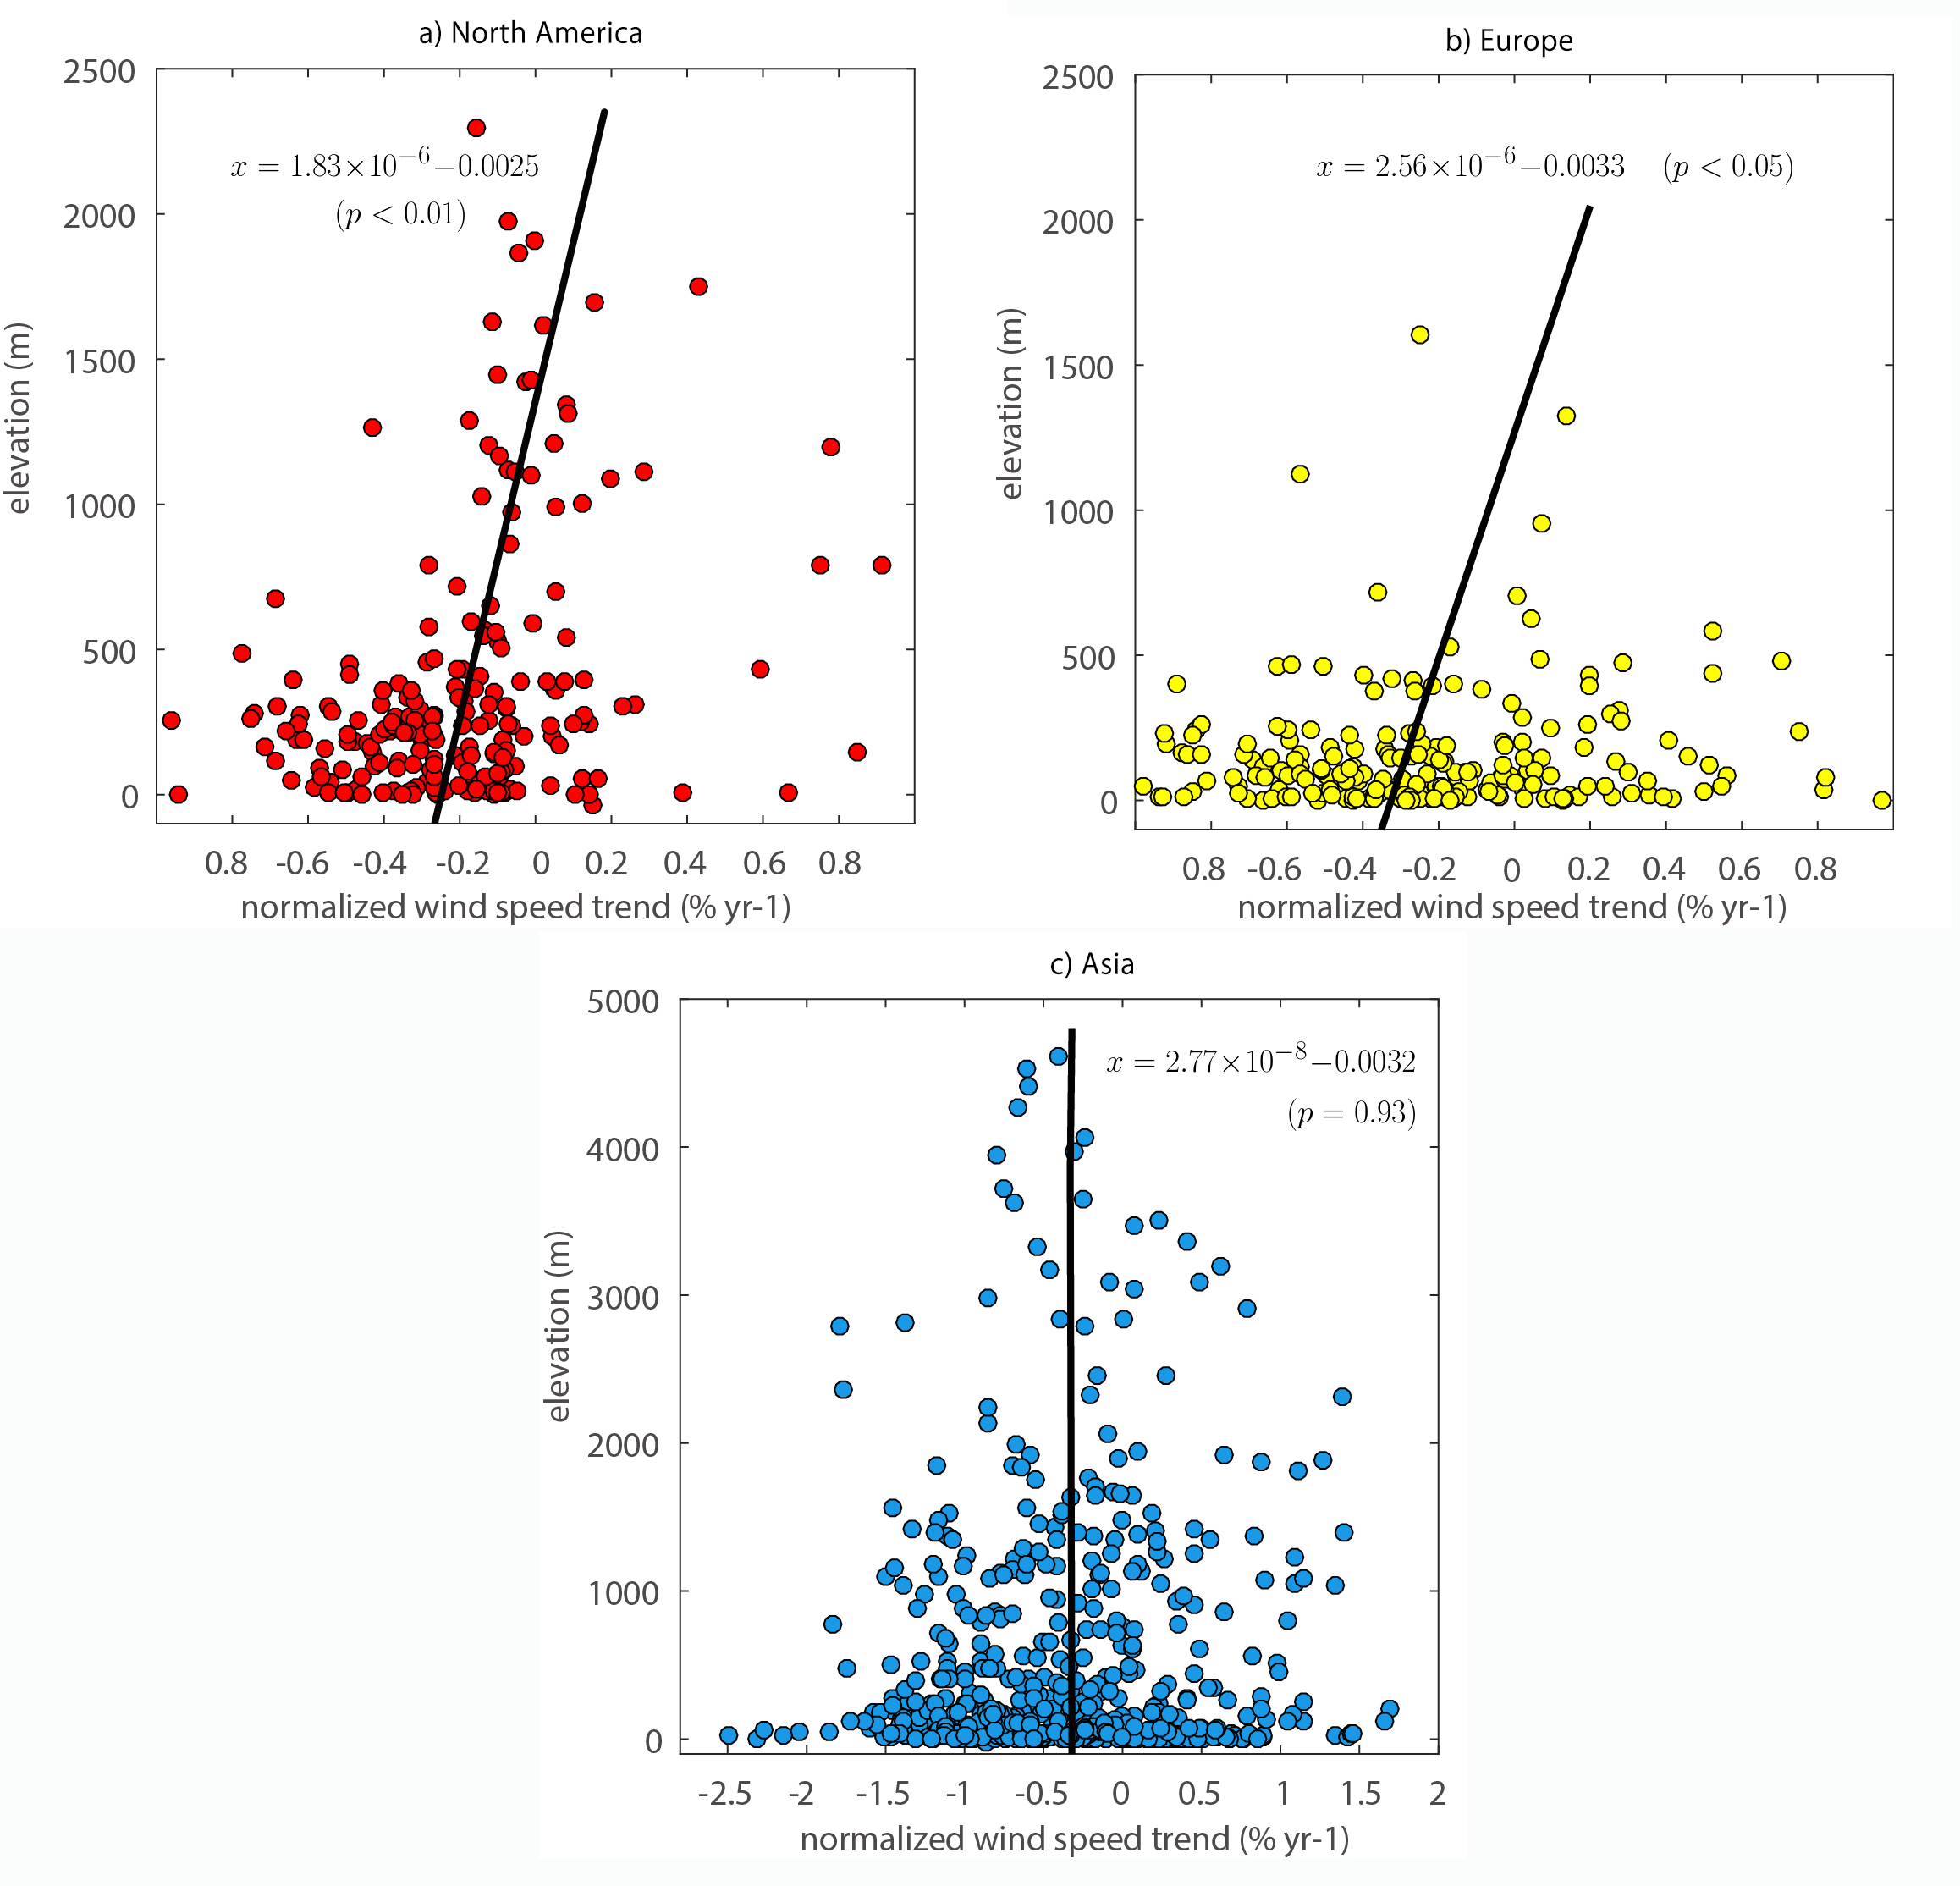
\includegraphics[width=0.75\textwidth]{各大洲归一化风速趋势与海拔的关系}
    \bicaption{各大洲归一化风速趋势与海拔的关系。a)北美洲,b)欧洲,c)亚洲。}{Normalized wind speed trends versus elevation in every continent. a)North America, b)Europe, c)Asia.}
    \label{fig:regionalwindvselevation}
\end{figure}

\section{北半球陆地地表风速趋势的年代际变化}

全球以及各大洲陆地地表风速趋势在不同年代际表现出了不同特征。全球平均来看,年平均风速趋势在2007年前后发生了一次显著变化(滑动t检验去趋势序列 p < 0.01,本段以下所提到年代际突变均采用此种方式计算得到),1979-2007年的趋势为-0.092 $m ~ s^{-1}$每十年,2007-2016年无明显趋势。这种年代际变化由夏、秋、冬季贡献,春季几乎没有体现出2007年后趋势减弱的现象(图 \ref{fig:regionalmedianwinddecadalchange} a))。在北美洲,年平均风速大致经历了1987年前平稳时期(无明显趋势),1987-2000缓慢下降时期(-0.059 $m ~ s^{-1}$每十年),2000-2010快速下降时期(-0.160 $m ~ s^{-1}$每十年)和2010年后平稳时期(无明显趋势)。1987年前风速较为平稳和2000-2010年快速下降在四季均有体现,而1987-2000四季表现差异较大,其中春季和夏季风速较为平稳,而秋季和冬季风速明显下降,2010年后夏、秋季风速出现上升,春、冬季风速继续下降(图 \ref{fig:regionalmedianwinddecadalchange} b))。在欧洲,年平均风速经历了1990年前快速下降(-0.254 $m ~ s^{-1}$每十年),1990-2000中速下降(-0.131 $m ~ s^{-1}$每十年)和2000年后缓慢下降(-0.072 $m ~ s^{-1}$每十年)三个时期。冬季风速突变点大致与年平均风速相同,而春季和秋季经历了两个时期,即快速下降和缓慢下降时期,突变点分别在2000和1993年。夏季最为特殊,2000年前风速下降,其后风速逐渐上升,2010年后趋于平稳(图 \ref{fig:regionalmedianwinddecadalchange} c))。在亚洲,年平均风速在1990年前快速下降(-0.190 $m ~ s^{-1}$每十年),1990-1997年趋于平稳 (无明显趋势),1997-2007再次快速下降(-0.206 $m ~ s^{-1}$每十年),2007年后再次趋于平稳(无明显趋势)。夏季和秋季风速与年平均风速年代际变化较为吻合,春季和冬季在2007年后年代际特征与年平均风速较为一致,2007年后有明显下降(图 \ref{fig:regionalmedianwinddecadalchange} d))。全球年平均风速的中位数在2007年前的减慢趋势在三个大洲均有体现,而2007年后的风速变为平稳的现象主要由北美洲和亚洲贡献,欧洲在2007年后依然保持了下降的趋势。

\begin{figure}[!ht]
    \centering
    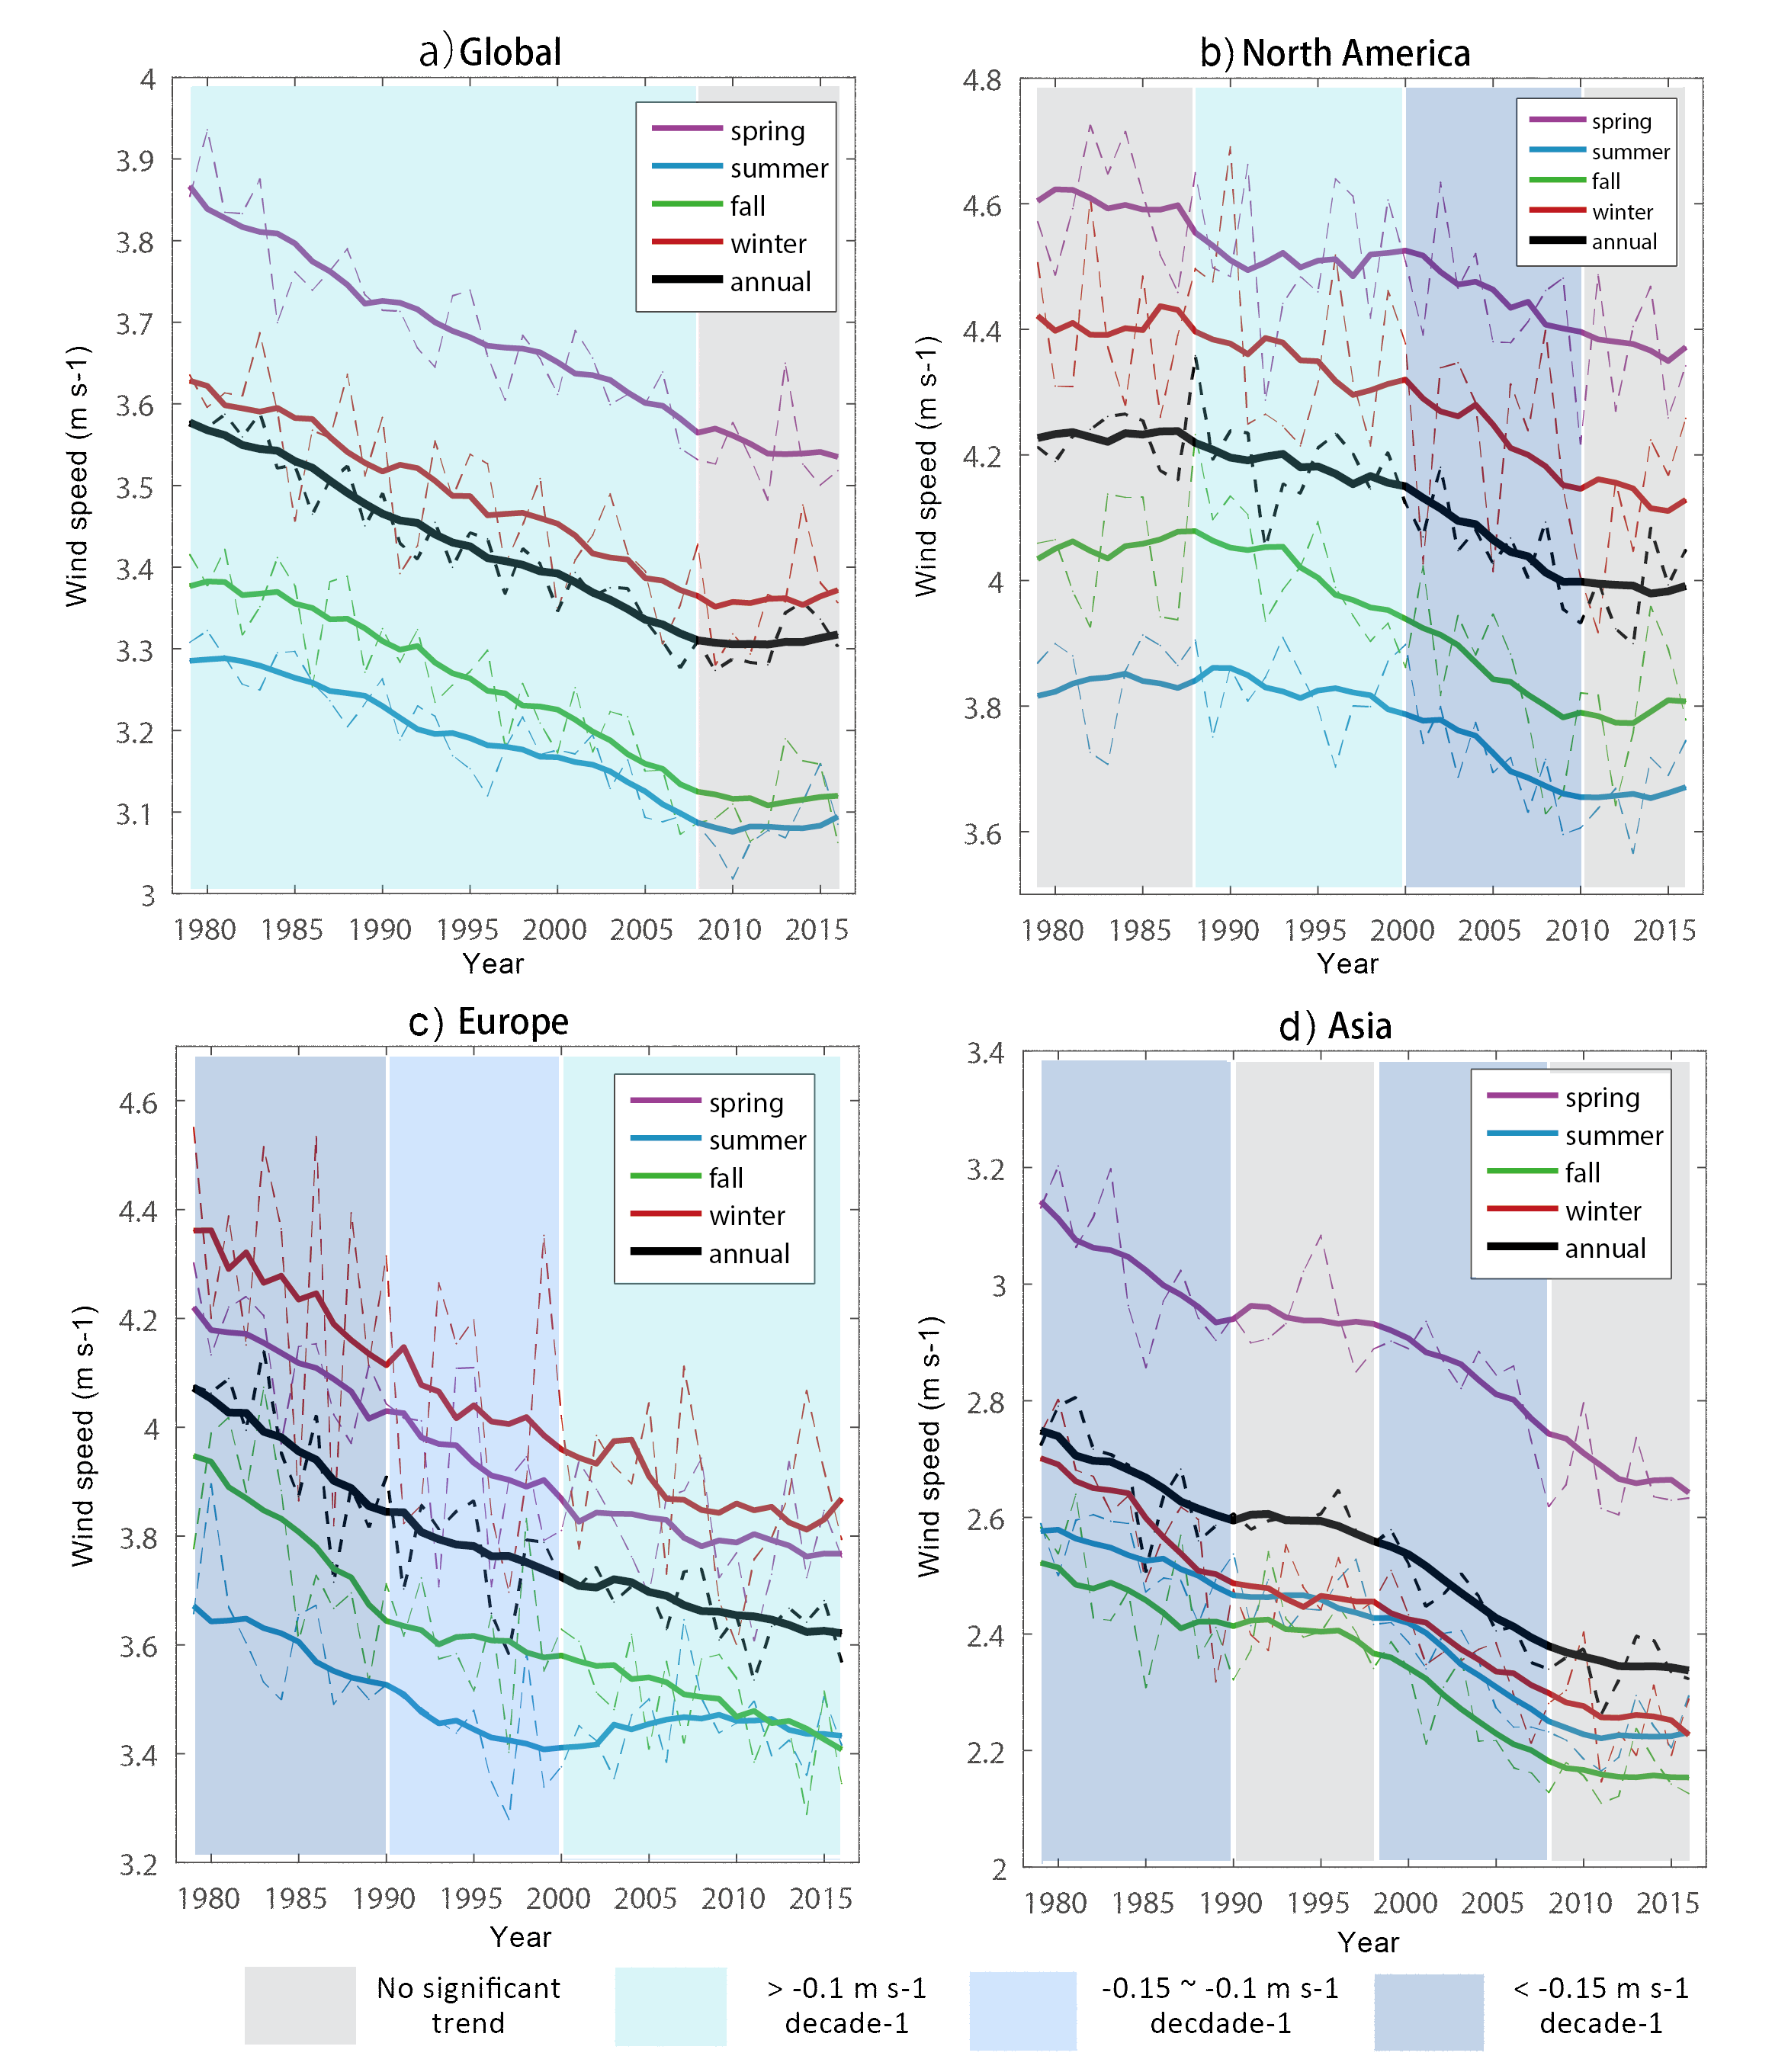
\includegraphics[width=0.9\textwidth]{各大洲中位数风速年代际演变}
    \bicaption{各大洲中位数风速年代际演变。a)全球,b)北美,c)欧洲,d)亚洲。紫色为春季,蓝色为夏季,绿色为秋季,红色为冬季,黑色为年平均。虚线为各年对应值,实线为虚线9点平滑的结果。底色为灰色、浅蓝、蓝色、深蓝的时段分别代表年平均风速无明显趋势、慢速下降、中速下降和快速下降。}{Decadal evolution of global and regional median wind speeds.  a)Global, b)North America, c)Europe, d)Asia. Purple color denotes spring, blue denotes summer, green denotes fall, red denotes winter, black denotes annual mean. Dash line denotes value for every year, soild line is 9-point moving mean of dash line. Periods with grey, light blue, blue, dark blue represent time when annual mean wind speeds have no trend, go down slowly, go down with medium speed, go down sharply, respectively.}
    \label{fig:regionalmedianwinddecadalchange}
\end{figure}

\section{北半球陆地地表风速长期变化的不确定性分析}

如第\ref{chap:intro}章所述,观测风速可能由于仪器更换、观测环境变化等,不能反映出真实的变化,尽管本章分析使用的风速序列经过了严格质量控制,依然不能完全排除上述人为因素的影响。为此,使用NCEP/NCAR、NCEP-DOE、ERA-Interim、JRA-55和MERRA-2等5套再分析资料再次计算陆地地表风速的长期变化,并与观测进行对比。值得一提的是,除JRA-55外,其他4套再分析资料均没有同化陆地地表风速观测。以下分析基于5套再分析资料10 $m$ U、V风场计算的年平均风速插值到观测点的结果。

\subsection{风速长期线性趋势的不确定性}

\begin{figure}[!t]
    \centering
    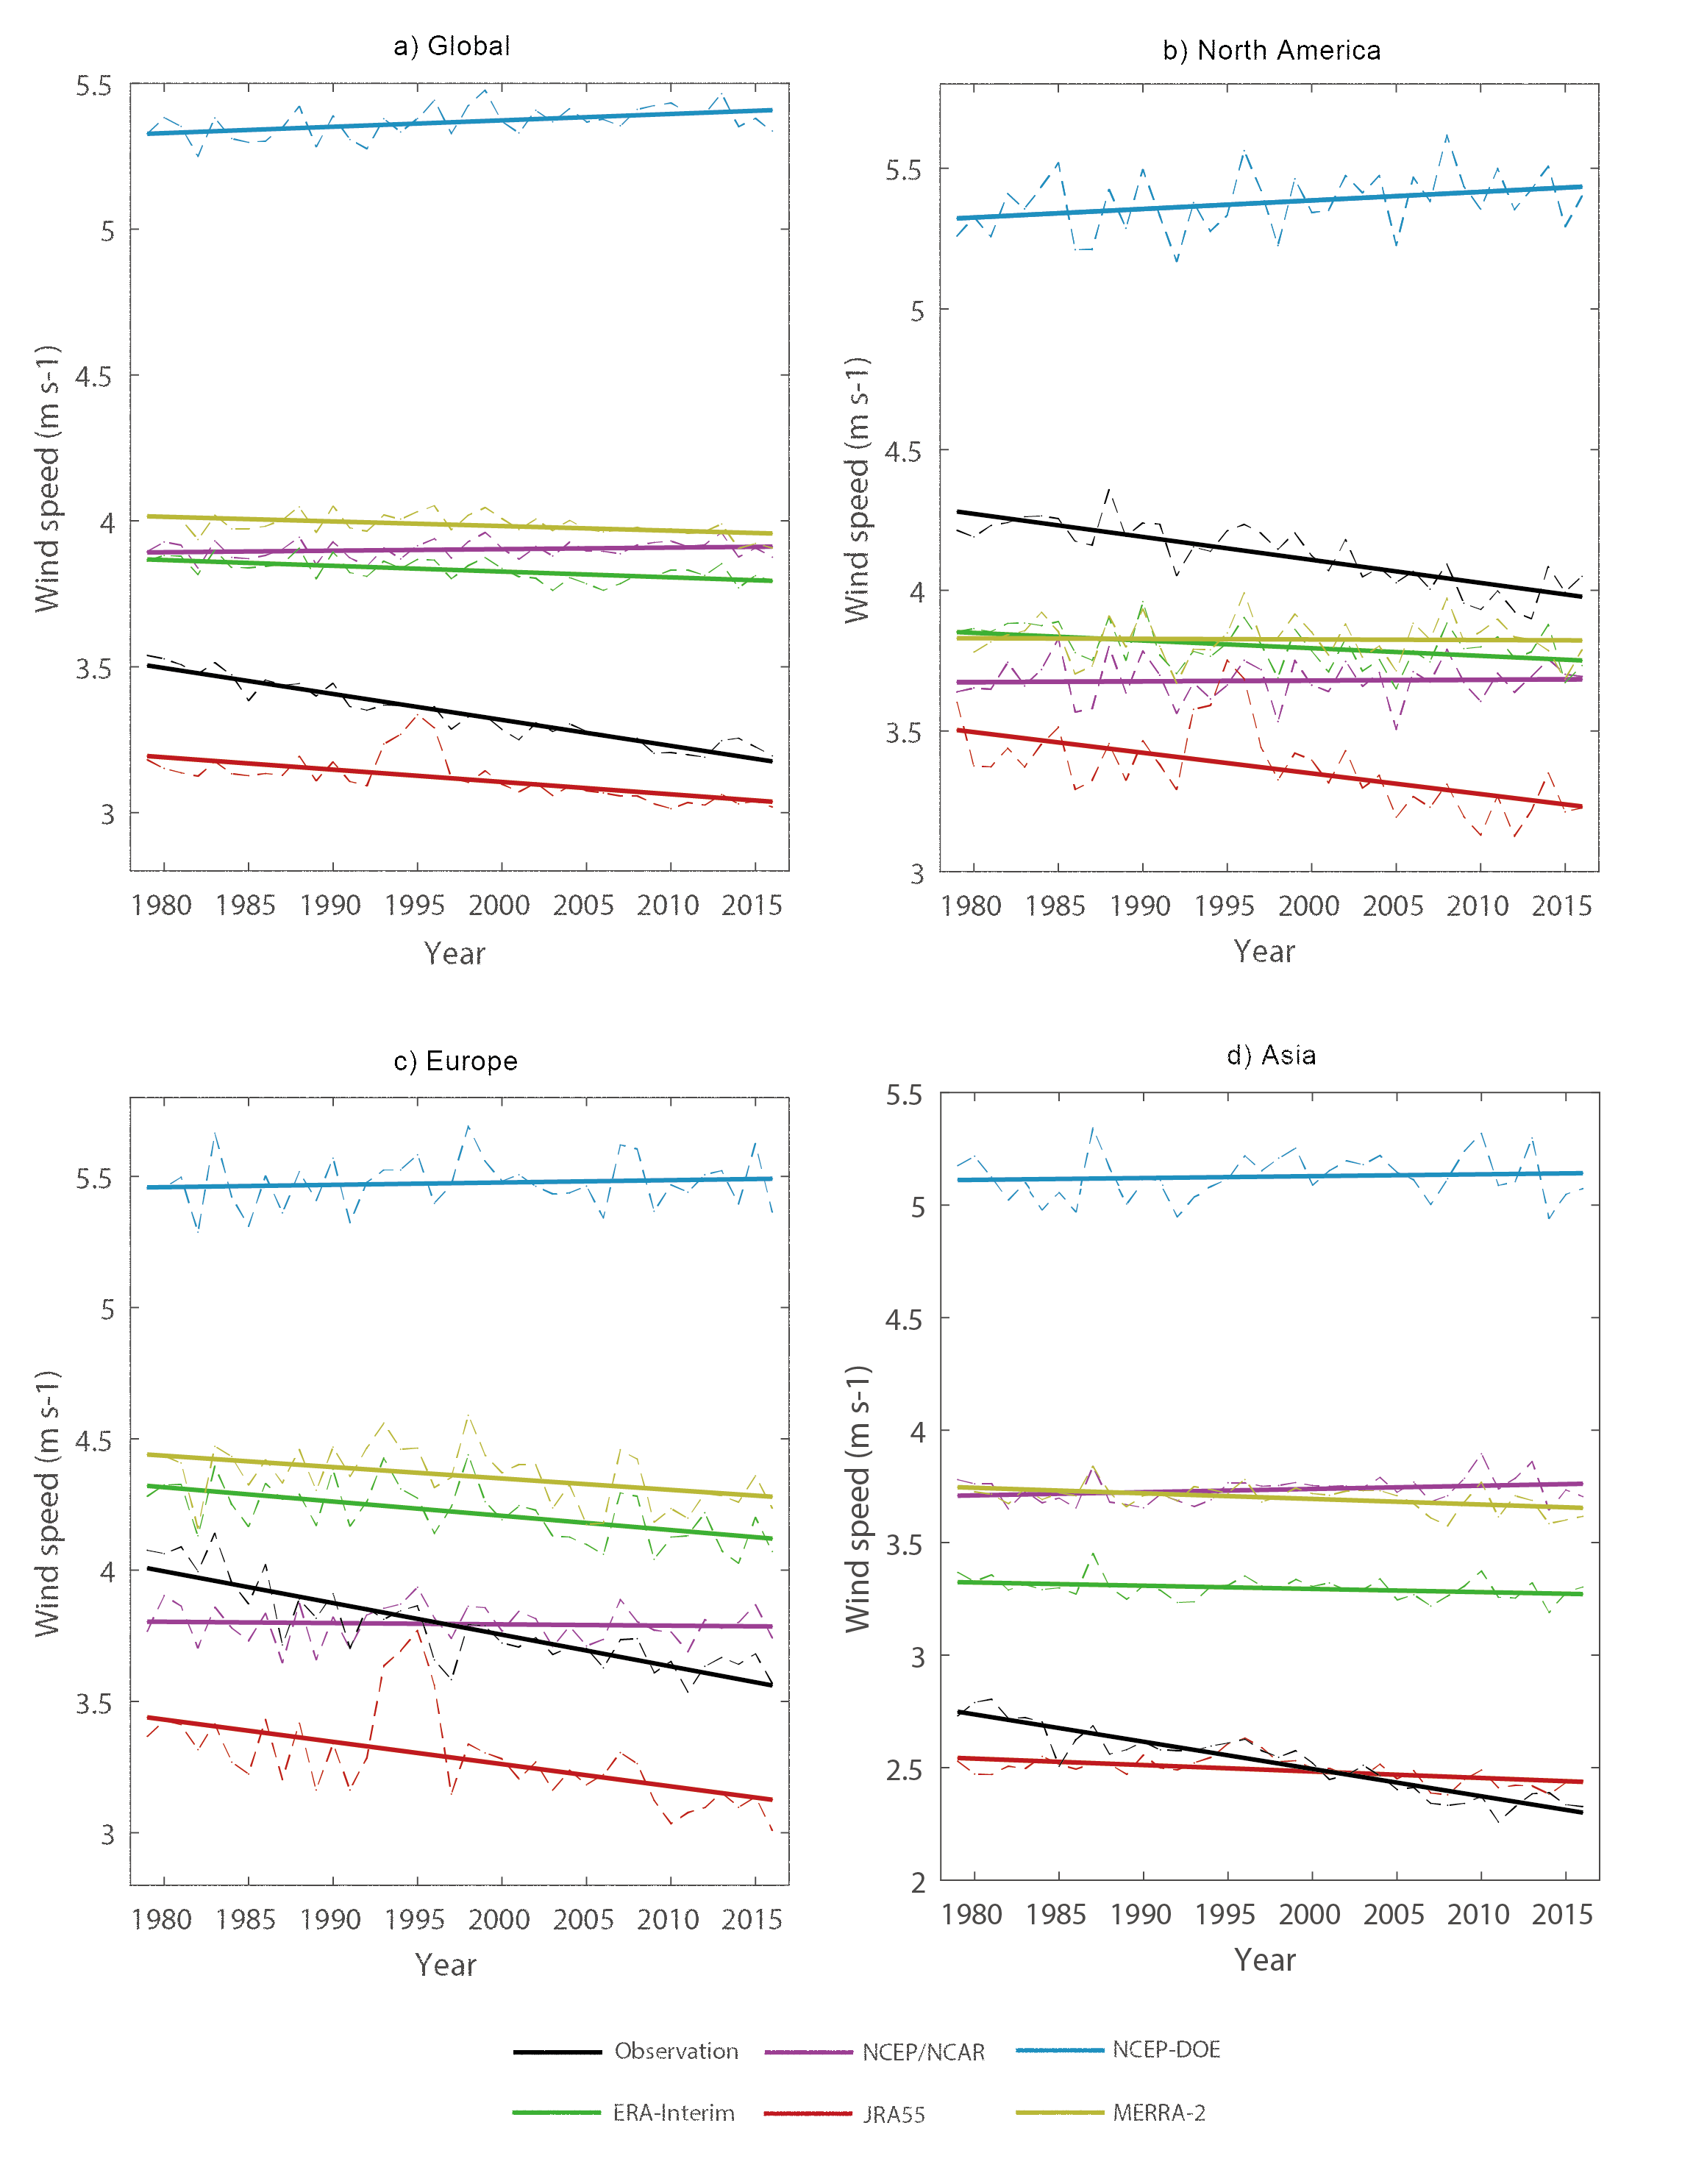
\includegraphics[width=0.9\textwidth]{风速趋势不确定性}
    \bicaption{观测及再分析资料风速长期线性趋势。a)全球,b)北美洲,c)欧洲,d)亚洲。虚线为年均值,实线为虚线的线性趋势。}{Wind speed trends in observation and reanalysis data. a)Global, b)North America, c) Europe, d)Asia. Dash line is annual mean value, solid line is linear trend line of dash line.}
    \label{fig:uncertaintywindtrend}
\end{figure}

全球平均风速上,NCEP-DOE风速明显偏大,与其他4套再分析资料及观测相差大于1 $m ~ s^{-1}$,NCEP/NCAR、ERA-Interim和MERRA-2非常接近,且都略大于观测(差别约0.5 $m ~ s^{-1}$),而JRA-55略小于观测(差别约0.3 $m ~ s^{-1}$)。风速长期趋势上,NCEP-DOE和ERA-Interim呈微弱上升趋势,分别为0.022和0.020 $m ~ s^{-1}$每十年;NCEP/NCAR无明显趋势;MERRA-2、JRA-55都呈现出下降趋势,分别为-0.016和-0.042 $m ~ s^{-1}$每十年,然而它们的下降速度都不及观测(-0.081 $m ~ s^{-1}$每十年)(图 \ref{fig:uncertaintywindtrend} a))。在北美洲,平均风速NCEP-DOE最大,其他4套再分析资料均小于观测,JRA-55最小。风速长期趋势上,NCEP-DOE风速以0.03 $m ~ s^{-1}$每十年的趋势上升,MERRA-2和NCEP/NCAR基本不变,ERA-Interim和JRA-55分别以-0.027和-0.073 $m ~ s^{-1}$每十年的趋势下降,观测风速趋势为-0.075 $m ~ s^{-1}$每十年(图 \ref{fig:uncertaintywindtrend} b))。在欧洲,平均风速除NCEP-DOE偏大外,MERRA-2和ERA-Interim略大于观测,JRA-55略小于观测,NCEP/NCAR与观测接近。风速趋势NCEP/NCAR与NCEP-DOE无明显趋势,其余3套再分析资料均呈下降趋势(ERA-Inteirm:-0.054 $m ~ s^{-1}$每十年,JRA-55:-0.085 $m ~ s^{-1}$每十年,MERRA-2:-0.043 $m ~ s^{-1}$每十年),观测风速趋势为-0.105 $m ~ s^{-1}$每十年(图 \ref{fig:uncertaintywindtrend} c))。在亚洲,平均风速除JRA-55与观测接近外其他均大于观测,NCEP-DOE差别最为显著(> 2 $m ~ s^{-1}$)。风速趋势ERA-Interim、JRA-55、MERAA-2和观测均为负值,分别为-0.014、-0.029、-0.025和-0.075 $m ~ s^{-1}$每十年,而NCEP/NCAR和NCEP-DOE无明显趋势(图 \ref{fig:uncertaintywindtrend} d))。


\subsection{风速趋势年代际变化的不确定性}

\begin{figure}[!b]
    \centering
    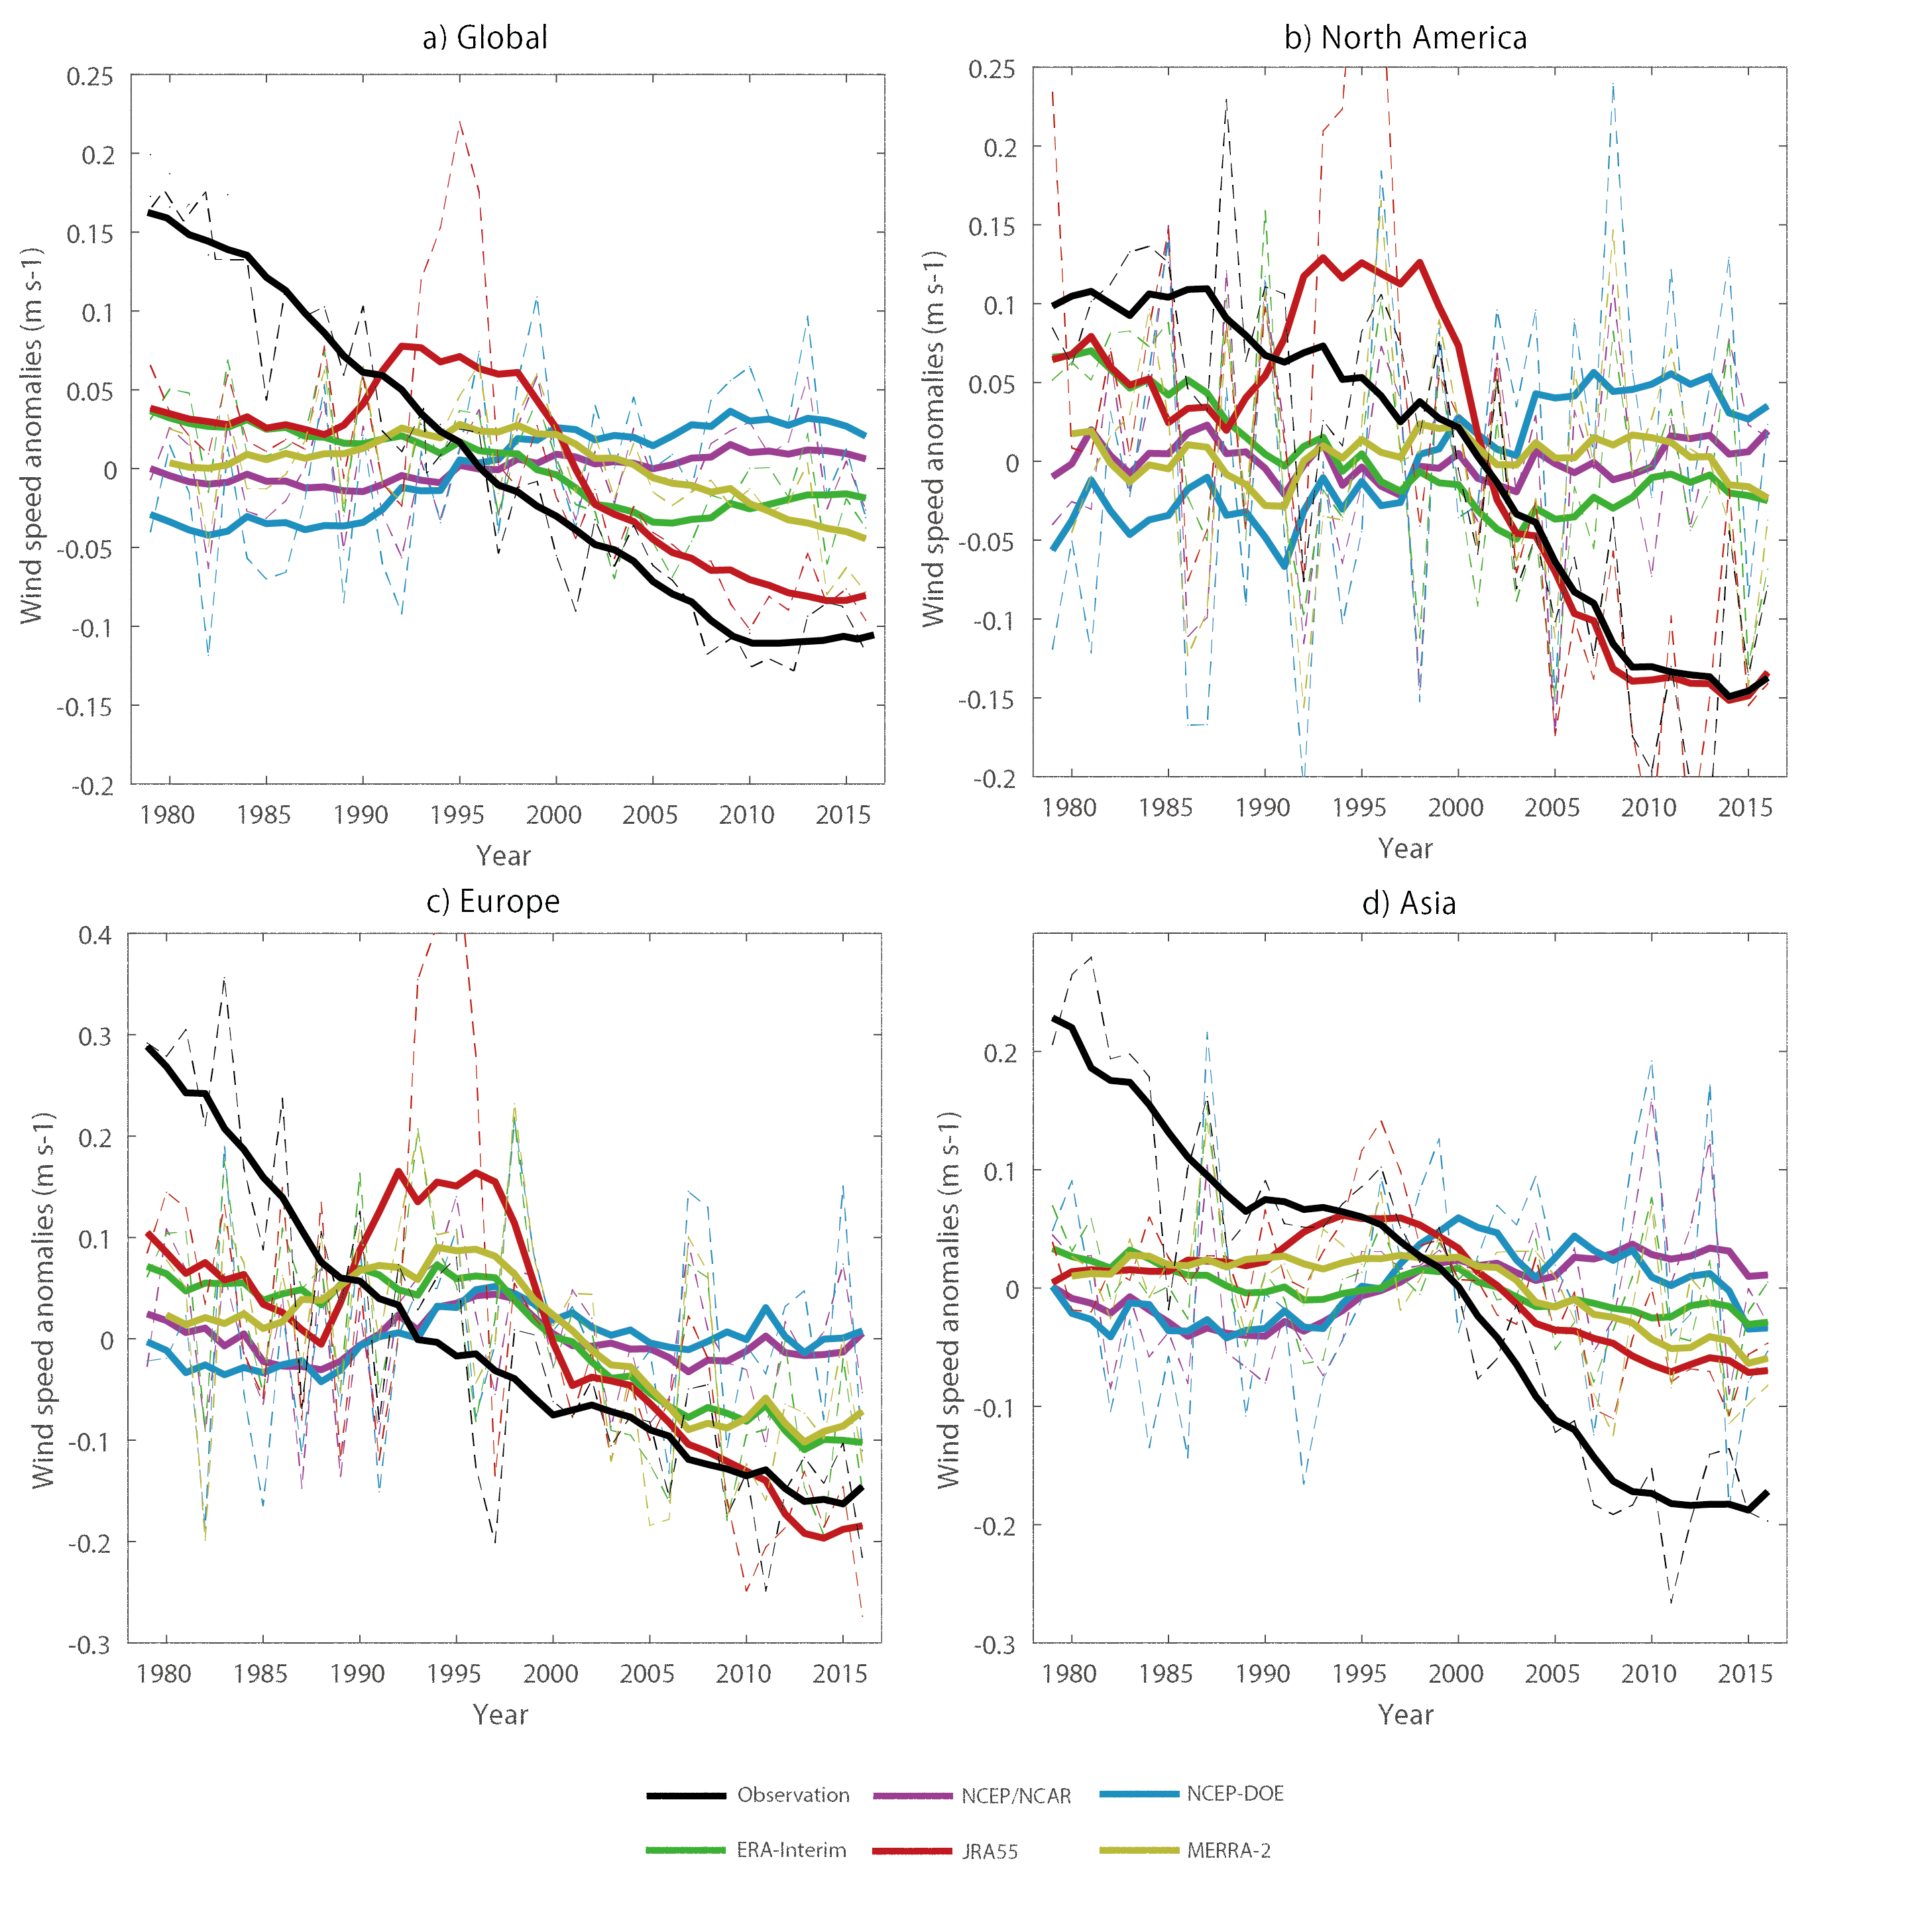
\includegraphics[width=0.9\textwidth]{风速年代际变化不确定性}
    \bicaption{观测及再分析资料风速年代际变化。a)全球,b)北美洲,c)欧洲,d)亚洲。虚线为年均值,实线为虚线9点平滑后的结果。}{Decadal changes of wind speed in observation and reanalysis data. a)Global, b)North America, c) Europe, d)Asia. Dash line is annual mean value, soild line is 9-point moving mean of dash line.}
    \label{fig:uncertaintywinddecadalchange}
\end{figure}

不同资料年平均风速年代际变化呈现的特点大不相同。全球平均来看,NCEP/NCAR和NCEP-DOE在1992-2000年期间风速有上升,1992年前和2000年后风速较为平稳;ERA-Interim在1995年前缓慢下降,1995-2005快速下降且下降速度与同期观测接近,2005年后风速回升;MERRA-2在1997年前风速上升而气候开始下降;JRA-55在1988年前缓慢下降,与同期ERA-Interim下降速度几乎一致,1988-2001年风速经历异常的极速上升,缓慢下降和异常的极速下降,后又快速下降,并且在2001-2007年下降速度与观测类似,其中1990年和2000年前后的极速上升和下降非常可能是由于JRA-55自身的错误所致,若将其扣除,JRA-55在1979-2016年间均呈下降趋势,2000年前下降较慢,其后下降较快(图 \ref{fig:uncertaintywinddecadalchange} a))。在北美洲,NCEP/NCAR和MERRA-2风速始终较为平稳;NCEP-DOE在1994年前和2005年后风速无显著趋势,1994-2005年间风速逐渐上升;ERA-Interim在2003年前风速下降而其后风速有上升趋势;JRA-55若扣除1990和2000前后的异常变化,表现为2000年前缓慢下降,2000-2010年快速下降,2010年后趋于平稳,与观测非常接近(图 \ref{fig:uncertaintywinddecadalchange} b))。在欧洲,NCEP/NCAR在1988年前风速缓慢下降,1988-1998风速上升,1988-2005风速再次缓慢下降,2005年后趋于平稳;NCEP-DOE与NCEP/NCAR年代际变化非常类似,不同之处在于NCEP-DOE在1988年前风速平稳;MERRA-2年代际变化也与NCEP/NCAR几乎一致除了1988-2005风速下降快于NCEP/NCAR;ERA-Interim在1995年前风速较为平稳,其后风速快速下降;JRA-55若扣除异常上升和下降,在1990年前快速下降,1990-2000趋于平稳,其后又快速下降(图 \ref{fig:uncertaintywinddecadalchange} c))。在亚洲,NCEP/NCAR在1998年前风速平稳,1998-2000风速上升,2000年后再次趋于平稳;NCEP-DOE前两个阶段与NCEP/NCAR接近,2000年后风速缓慢下降;ERA-Interim在1998年前风速缓慢下降,1995-2005缓慢上升后又缓慢下降,2005年后趋于平稳;MERRA-2在2000年前风速平稳,2000年后缓慢下降;JRA-55在1990年和2000年风速异常变化相对较小,扣除之后整体上体现为2000年前平稳,2000-2010缓慢下降,2010年后再次平稳(图 \ref{fig:uncertaintywinddecadalchange} d))。


\section{本章小结}

本章利用观测数据分析了全球(由于数据绝大多数来源于北半球,所以主要体现的是北半球的特征)以及北美洲、欧洲和亚洲分别的陆地地表风速长期趋势和趋势的年代际变化,并讨论了其中的不确定性,得到以下结论:

\begin{enumerate}

\item 陆地地表风速减弱是全球(主要是北半球)普遍发生的现象,中位数风速趋势为-0.081 $m ~ s^{-1}$每十年,北美洲、欧洲和亚洲分别为-0.075,-0.105和-0.075 $m ~ s^{-1}$每十年。美国中北和东北部,中国东北,西欧和东欧风速下降最为明显。

\item 风速趋势在不同百分位风速的表现有一定差别,总体来看,高百分位风速下降快于低百分位,但北美洲例外,其低百分位风速下降明显高于高百分位。

\item 风速趋势有明显的季节差异,总体来看,春季下降最快而夏季下降最慢。

\item 不同海拔的风速趋势有所差异,在北美洲和欧洲,海拔越高风速趋势越趋向于正,亚洲海拔与风速趋势无显著相关。

\item 风速趋势有显著的年代际变化。总体来看,风速下降发生在2010年前,之后风速趋于平稳。北美洲风速下降出现在1980至2010年间,其他时间风速平稳;欧洲近38年风速持续下降,2000年之后下降慢于之前;亚洲风速下降发生在1990年前和1997-2007年间,其他时间风速平稳。在不同季节上的风速年代际变化大多与年均值一致,但欧洲夏季与其他季节差异明显,表现为2000年后显著增加。

\item 使用5套再分析资料得到的中位数风速趋势从0.022 $m ~ s^{-1}$每十年至-0.042 $m ~ s^{-1}$每十年不等,年代际变化也有较明显的不一致性,其中唯一同化了陆地地表风速观测的再分析资料JRA-55与观测的长期变化最为接近。
\end{enumerate}
